
% Default to the notebook output style

    


% Inherit from the specified cell style.




    
\documentclass[11pt]{article}

    
    
    \usepackage[T1]{fontenc}
    % Nicer default font (+ math font) than Computer Modern for most use cases
    \usepackage{mathpazo}

    % Basic figure setup, for now with no caption control since it's done
    % automatically by Pandoc (which extracts ![](path) syntax from Markdown).
    \usepackage{graphicx}
    % We will generate all images so they have a width \maxwidth. This means
    % that they will get their normal width if they fit onto the page, but
    % are scaled down if they would overflow the margins.
    \makeatletter
    \def\maxwidth{\ifdim\Gin@nat@width>\linewidth\linewidth
    \else\Gin@nat@width\fi}
    \makeatother
    \let\Oldincludegraphics\includegraphics
    % Set max figure width to be 80% of text width, for now hardcoded.
    \renewcommand{\includegraphics}[1]{\Oldincludegraphics[width=.8\maxwidth]{#1}}
    % Ensure that by default, figures have no caption (until we provide a
    % proper Figure object with a Caption API and a way to capture that
    % in the conversion process - todo).
    \usepackage{caption}
    \DeclareCaptionLabelFormat{nolabel}{}
    \captionsetup{labelformat=nolabel}

    \usepackage{adjustbox} % Used to constrain images to a maximum size 
    \usepackage{xcolor} % Allow colors to be defined
    \usepackage{enumerate} % Needed for markdown enumerations to work
    \usepackage{geometry} % Used to adjust the document margins
    \usepackage{amsmath} % Equations
    \usepackage{amssymb} % Equations
    \usepackage{textcomp} % defines textquotesingle
    % Hack from http://tex.stackexchange.com/a/47451/13684:
    \AtBeginDocument{%
        \def\PYZsq{\textquotesingle}% Upright quotes in Pygmentized code
    }
    \usepackage{upquote} % Upright quotes for verbatim code
    \usepackage{eurosym} % defines \euro
    \usepackage[mathletters]{ucs} % Extended unicode (utf-8) support
    \usepackage[utf8x]{inputenc} % Allow utf-8 characters in the tex document
    \usepackage{fancyvrb} % verbatim replacement that allows latex
    \usepackage{grffile} % extends the file name processing of package graphics 
                         % to support a larger range 
    % The hyperref package gives us a pdf with properly built
    % internal navigation ('pdf bookmarks' for the table of contents,
    % internal cross-reference links, web links for URLs, etc.)
    \usepackage{hyperref}
    \usepackage{longtable} % longtable support required by pandoc >1.10
    \usepackage{booktabs}  % table support for pandoc > 1.12.2
    \usepackage[inline]{enumitem} % IRkernel/repr support (it uses the enumerate* environment)
    \usepackage[normalem]{ulem} % ulem is needed to support strikethroughs (\sout)
                                % normalem makes italics be italics, not underlines
    

    
    
    % Colors for the hyperref package
    \definecolor{urlcolor}{rgb}{0,.145,.698}
    \definecolor{linkcolor}{rgb}{.71,0.21,0.01}
    \definecolor{citecolor}{rgb}{.12,.54,.11}

    % ANSI colors
    \definecolor{ansi-black}{HTML}{3E424D}
    \definecolor{ansi-black-intense}{HTML}{282C36}
    \definecolor{ansi-red}{HTML}{E75C58}
    \definecolor{ansi-red-intense}{HTML}{B22B31}
    \definecolor{ansi-green}{HTML}{00A250}
    \definecolor{ansi-green-intense}{HTML}{007427}
    \definecolor{ansi-yellow}{HTML}{DDB62B}
    \definecolor{ansi-yellow-intense}{HTML}{B27D12}
    \definecolor{ansi-blue}{HTML}{208FFB}
    \definecolor{ansi-blue-intense}{HTML}{0065CA}
    \definecolor{ansi-magenta}{HTML}{D160C4}
    \definecolor{ansi-magenta-intense}{HTML}{A03196}
    \definecolor{ansi-cyan}{HTML}{60C6C8}
    \definecolor{ansi-cyan-intense}{HTML}{258F8F}
    \definecolor{ansi-white}{HTML}{C5C1B4}
    \definecolor{ansi-white-intense}{HTML}{A1A6B2}

    % commands and environments needed by pandoc snippets
    % extracted from the output of `pandoc -s`
    \providecommand{\tightlist}{%
      \setlength{\itemsep}{0pt}\setlength{\parskip}{0pt}}
    \DefineVerbatimEnvironment{Highlighting}{Verbatim}{commandchars=\\\{\}}
    % Add ',fontsize=\small' for more characters per line
    \newenvironment{Shaded}{}{}
    \newcommand{\KeywordTok}[1]{\textcolor[rgb]{0.00,0.44,0.13}{\textbf{{#1}}}}
    \newcommand{\DataTypeTok}[1]{\textcolor[rgb]{0.56,0.13,0.00}{{#1}}}
    \newcommand{\DecValTok}[1]{\textcolor[rgb]{0.25,0.63,0.44}{{#1}}}
    \newcommand{\BaseNTok}[1]{\textcolor[rgb]{0.25,0.63,0.44}{{#1}}}
    \newcommand{\FloatTok}[1]{\textcolor[rgb]{0.25,0.63,0.44}{{#1}}}
    \newcommand{\CharTok}[1]{\textcolor[rgb]{0.25,0.44,0.63}{{#1}}}
    \newcommand{\StringTok}[1]{\textcolor[rgb]{0.25,0.44,0.63}{{#1}}}
    \newcommand{\CommentTok}[1]{\textcolor[rgb]{0.38,0.63,0.69}{\textit{{#1}}}}
    \newcommand{\OtherTok}[1]{\textcolor[rgb]{0.00,0.44,0.13}{{#1}}}
    \newcommand{\AlertTok}[1]{\textcolor[rgb]{1.00,0.00,0.00}{\textbf{{#1}}}}
    \newcommand{\FunctionTok}[1]{\textcolor[rgb]{0.02,0.16,0.49}{{#1}}}
    \newcommand{\RegionMarkerTok}[1]{{#1}}
    \newcommand{\ErrorTok}[1]{\textcolor[rgb]{1.00,0.00,0.00}{\textbf{{#1}}}}
    \newcommand{\NormalTok}[1]{{#1}}
    
    % Additional commands for more recent versions of Pandoc
    \newcommand{\ConstantTok}[1]{\textcolor[rgb]{0.53,0.00,0.00}{{#1}}}
    \newcommand{\SpecialCharTok}[1]{\textcolor[rgb]{0.25,0.44,0.63}{{#1}}}
    \newcommand{\VerbatimStringTok}[1]{\textcolor[rgb]{0.25,0.44,0.63}{{#1}}}
    \newcommand{\SpecialStringTok}[1]{\textcolor[rgb]{0.73,0.40,0.53}{{#1}}}
    \newcommand{\ImportTok}[1]{{#1}}
    \newcommand{\DocumentationTok}[1]{\textcolor[rgb]{0.73,0.13,0.13}{\textit{{#1}}}}
    \newcommand{\AnnotationTok}[1]{\textcolor[rgb]{0.38,0.63,0.69}{\textbf{\textit{{#1}}}}}
    \newcommand{\CommentVarTok}[1]{\textcolor[rgb]{0.38,0.63,0.69}{\textbf{\textit{{#1}}}}}
    \newcommand{\VariableTok}[1]{\textcolor[rgb]{0.10,0.09,0.49}{{#1}}}
    \newcommand{\ControlFlowTok}[1]{\textcolor[rgb]{0.00,0.44,0.13}{\textbf{{#1}}}}
    \newcommand{\OperatorTok}[1]{\textcolor[rgb]{0.40,0.40,0.40}{{#1}}}
    \newcommand{\BuiltInTok}[1]{{#1}}
    \newcommand{\ExtensionTok}[1]{{#1}}
    \newcommand{\PreprocessorTok}[1]{\textcolor[rgb]{0.74,0.48,0.00}{{#1}}}
    \newcommand{\AttributeTok}[1]{\textcolor[rgb]{0.49,0.56,0.16}{{#1}}}
    \newcommand{\InformationTok}[1]{\textcolor[rgb]{0.38,0.63,0.69}{\textbf{\textit{{#1}}}}}
    \newcommand{\WarningTok}[1]{\textcolor[rgb]{0.38,0.63,0.69}{\textbf{\textit{{#1}}}}}
    
    
    % Define a nice break command that doesn't care if a line doesn't already
    % exist.
    \def\br{\hspace*{\fill} \\* }
    % Math Jax compatability definitions
    \def\gt{>}
    \def\lt{<}
    % Document parameters
    \title{h4-smoada}
    
    
    

    % Pygments definitions
    
\makeatletter
\def\PY@reset{\let\PY@it=\relax \let\PY@bf=\relax%
    \let\PY@ul=\relax \let\PY@tc=\relax%
    \let\PY@bc=\relax \let\PY@ff=\relax}
\def\PY@tok#1{\csname PY@tok@#1\endcsname}
\def\PY@toks#1+{\ifx\relax#1\empty\else%
    \PY@tok{#1}\expandafter\PY@toks\fi}
\def\PY@do#1{\PY@bc{\PY@tc{\PY@ul{%
    \PY@it{\PY@bf{\PY@ff{#1}}}}}}}
\def\PY#1#2{\PY@reset\PY@toks#1+\relax+\PY@do{#2}}

\expandafter\def\csname PY@tok@w\endcsname{\def\PY@tc##1{\textcolor[rgb]{0.73,0.73,0.73}{##1}}}
\expandafter\def\csname PY@tok@c\endcsname{\let\PY@it=\textit\def\PY@tc##1{\textcolor[rgb]{0.25,0.50,0.50}{##1}}}
\expandafter\def\csname PY@tok@cp\endcsname{\def\PY@tc##1{\textcolor[rgb]{0.74,0.48,0.00}{##1}}}
\expandafter\def\csname PY@tok@k\endcsname{\let\PY@bf=\textbf\def\PY@tc##1{\textcolor[rgb]{0.00,0.50,0.00}{##1}}}
\expandafter\def\csname PY@tok@kp\endcsname{\def\PY@tc##1{\textcolor[rgb]{0.00,0.50,0.00}{##1}}}
\expandafter\def\csname PY@tok@kt\endcsname{\def\PY@tc##1{\textcolor[rgb]{0.69,0.00,0.25}{##1}}}
\expandafter\def\csname PY@tok@o\endcsname{\def\PY@tc##1{\textcolor[rgb]{0.40,0.40,0.40}{##1}}}
\expandafter\def\csname PY@tok@ow\endcsname{\let\PY@bf=\textbf\def\PY@tc##1{\textcolor[rgb]{0.67,0.13,1.00}{##1}}}
\expandafter\def\csname PY@tok@nb\endcsname{\def\PY@tc##1{\textcolor[rgb]{0.00,0.50,0.00}{##1}}}
\expandafter\def\csname PY@tok@nf\endcsname{\def\PY@tc##1{\textcolor[rgb]{0.00,0.00,1.00}{##1}}}
\expandafter\def\csname PY@tok@nc\endcsname{\let\PY@bf=\textbf\def\PY@tc##1{\textcolor[rgb]{0.00,0.00,1.00}{##1}}}
\expandafter\def\csname PY@tok@nn\endcsname{\let\PY@bf=\textbf\def\PY@tc##1{\textcolor[rgb]{0.00,0.00,1.00}{##1}}}
\expandafter\def\csname PY@tok@ne\endcsname{\let\PY@bf=\textbf\def\PY@tc##1{\textcolor[rgb]{0.82,0.25,0.23}{##1}}}
\expandafter\def\csname PY@tok@nv\endcsname{\def\PY@tc##1{\textcolor[rgb]{0.10,0.09,0.49}{##1}}}
\expandafter\def\csname PY@tok@no\endcsname{\def\PY@tc##1{\textcolor[rgb]{0.53,0.00,0.00}{##1}}}
\expandafter\def\csname PY@tok@nl\endcsname{\def\PY@tc##1{\textcolor[rgb]{0.63,0.63,0.00}{##1}}}
\expandafter\def\csname PY@tok@ni\endcsname{\let\PY@bf=\textbf\def\PY@tc##1{\textcolor[rgb]{0.60,0.60,0.60}{##1}}}
\expandafter\def\csname PY@tok@na\endcsname{\def\PY@tc##1{\textcolor[rgb]{0.49,0.56,0.16}{##1}}}
\expandafter\def\csname PY@tok@nt\endcsname{\let\PY@bf=\textbf\def\PY@tc##1{\textcolor[rgb]{0.00,0.50,0.00}{##1}}}
\expandafter\def\csname PY@tok@nd\endcsname{\def\PY@tc##1{\textcolor[rgb]{0.67,0.13,1.00}{##1}}}
\expandafter\def\csname PY@tok@s\endcsname{\def\PY@tc##1{\textcolor[rgb]{0.73,0.13,0.13}{##1}}}
\expandafter\def\csname PY@tok@sd\endcsname{\let\PY@it=\textit\def\PY@tc##1{\textcolor[rgb]{0.73,0.13,0.13}{##1}}}
\expandafter\def\csname PY@tok@si\endcsname{\let\PY@bf=\textbf\def\PY@tc##1{\textcolor[rgb]{0.73,0.40,0.53}{##1}}}
\expandafter\def\csname PY@tok@se\endcsname{\let\PY@bf=\textbf\def\PY@tc##1{\textcolor[rgb]{0.73,0.40,0.13}{##1}}}
\expandafter\def\csname PY@tok@sr\endcsname{\def\PY@tc##1{\textcolor[rgb]{0.73,0.40,0.53}{##1}}}
\expandafter\def\csname PY@tok@ss\endcsname{\def\PY@tc##1{\textcolor[rgb]{0.10,0.09,0.49}{##1}}}
\expandafter\def\csname PY@tok@sx\endcsname{\def\PY@tc##1{\textcolor[rgb]{0.00,0.50,0.00}{##1}}}
\expandafter\def\csname PY@tok@m\endcsname{\def\PY@tc##1{\textcolor[rgb]{0.40,0.40,0.40}{##1}}}
\expandafter\def\csname PY@tok@gh\endcsname{\let\PY@bf=\textbf\def\PY@tc##1{\textcolor[rgb]{0.00,0.00,0.50}{##1}}}
\expandafter\def\csname PY@tok@gu\endcsname{\let\PY@bf=\textbf\def\PY@tc##1{\textcolor[rgb]{0.50,0.00,0.50}{##1}}}
\expandafter\def\csname PY@tok@gd\endcsname{\def\PY@tc##1{\textcolor[rgb]{0.63,0.00,0.00}{##1}}}
\expandafter\def\csname PY@tok@gi\endcsname{\def\PY@tc##1{\textcolor[rgb]{0.00,0.63,0.00}{##1}}}
\expandafter\def\csname PY@tok@gr\endcsname{\def\PY@tc##1{\textcolor[rgb]{1.00,0.00,0.00}{##1}}}
\expandafter\def\csname PY@tok@ge\endcsname{\let\PY@it=\textit}
\expandafter\def\csname PY@tok@gs\endcsname{\let\PY@bf=\textbf}
\expandafter\def\csname PY@tok@gp\endcsname{\let\PY@bf=\textbf\def\PY@tc##1{\textcolor[rgb]{0.00,0.00,0.50}{##1}}}
\expandafter\def\csname PY@tok@go\endcsname{\def\PY@tc##1{\textcolor[rgb]{0.53,0.53,0.53}{##1}}}
\expandafter\def\csname PY@tok@gt\endcsname{\def\PY@tc##1{\textcolor[rgb]{0.00,0.27,0.87}{##1}}}
\expandafter\def\csname PY@tok@err\endcsname{\def\PY@bc##1{\setlength{\fboxsep}{0pt}\fcolorbox[rgb]{1.00,0.00,0.00}{1,1,1}{\strut ##1}}}
\expandafter\def\csname PY@tok@kc\endcsname{\let\PY@bf=\textbf\def\PY@tc##1{\textcolor[rgb]{0.00,0.50,0.00}{##1}}}
\expandafter\def\csname PY@tok@kd\endcsname{\let\PY@bf=\textbf\def\PY@tc##1{\textcolor[rgb]{0.00,0.50,0.00}{##1}}}
\expandafter\def\csname PY@tok@kn\endcsname{\let\PY@bf=\textbf\def\PY@tc##1{\textcolor[rgb]{0.00,0.50,0.00}{##1}}}
\expandafter\def\csname PY@tok@kr\endcsname{\let\PY@bf=\textbf\def\PY@tc##1{\textcolor[rgb]{0.00,0.50,0.00}{##1}}}
\expandafter\def\csname PY@tok@bp\endcsname{\def\PY@tc##1{\textcolor[rgb]{0.00,0.50,0.00}{##1}}}
\expandafter\def\csname PY@tok@fm\endcsname{\def\PY@tc##1{\textcolor[rgb]{0.00,0.00,1.00}{##1}}}
\expandafter\def\csname PY@tok@vc\endcsname{\def\PY@tc##1{\textcolor[rgb]{0.10,0.09,0.49}{##1}}}
\expandafter\def\csname PY@tok@vg\endcsname{\def\PY@tc##1{\textcolor[rgb]{0.10,0.09,0.49}{##1}}}
\expandafter\def\csname PY@tok@vi\endcsname{\def\PY@tc##1{\textcolor[rgb]{0.10,0.09,0.49}{##1}}}
\expandafter\def\csname PY@tok@vm\endcsname{\def\PY@tc##1{\textcolor[rgb]{0.10,0.09,0.49}{##1}}}
\expandafter\def\csname PY@tok@sa\endcsname{\def\PY@tc##1{\textcolor[rgb]{0.73,0.13,0.13}{##1}}}
\expandafter\def\csname PY@tok@sb\endcsname{\def\PY@tc##1{\textcolor[rgb]{0.73,0.13,0.13}{##1}}}
\expandafter\def\csname PY@tok@sc\endcsname{\def\PY@tc##1{\textcolor[rgb]{0.73,0.13,0.13}{##1}}}
\expandafter\def\csname PY@tok@dl\endcsname{\def\PY@tc##1{\textcolor[rgb]{0.73,0.13,0.13}{##1}}}
\expandafter\def\csname PY@tok@s2\endcsname{\def\PY@tc##1{\textcolor[rgb]{0.73,0.13,0.13}{##1}}}
\expandafter\def\csname PY@tok@sh\endcsname{\def\PY@tc##1{\textcolor[rgb]{0.73,0.13,0.13}{##1}}}
\expandafter\def\csname PY@tok@s1\endcsname{\def\PY@tc##1{\textcolor[rgb]{0.73,0.13,0.13}{##1}}}
\expandafter\def\csname PY@tok@mb\endcsname{\def\PY@tc##1{\textcolor[rgb]{0.40,0.40,0.40}{##1}}}
\expandafter\def\csname PY@tok@mf\endcsname{\def\PY@tc##1{\textcolor[rgb]{0.40,0.40,0.40}{##1}}}
\expandafter\def\csname PY@tok@mh\endcsname{\def\PY@tc##1{\textcolor[rgb]{0.40,0.40,0.40}{##1}}}
\expandafter\def\csname PY@tok@mi\endcsname{\def\PY@tc##1{\textcolor[rgb]{0.40,0.40,0.40}{##1}}}
\expandafter\def\csname PY@tok@il\endcsname{\def\PY@tc##1{\textcolor[rgb]{0.40,0.40,0.40}{##1}}}
\expandafter\def\csname PY@tok@mo\endcsname{\def\PY@tc##1{\textcolor[rgb]{0.40,0.40,0.40}{##1}}}
\expandafter\def\csname PY@tok@ch\endcsname{\let\PY@it=\textit\def\PY@tc##1{\textcolor[rgb]{0.25,0.50,0.50}{##1}}}
\expandafter\def\csname PY@tok@cm\endcsname{\let\PY@it=\textit\def\PY@tc##1{\textcolor[rgb]{0.25,0.50,0.50}{##1}}}
\expandafter\def\csname PY@tok@cpf\endcsname{\let\PY@it=\textit\def\PY@tc##1{\textcolor[rgb]{0.25,0.50,0.50}{##1}}}
\expandafter\def\csname PY@tok@c1\endcsname{\let\PY@it=\textit\def\PY@tc##1{\textcolor[rgb]{0.25,0.50,0.50}{##1}}}
\expandafter\def\csname PY@tok@cs\endcsname{\let\PY@it=\textit\def\PY@tc##1{\textcolor[rgb]{0.25,0.50,0.50}{##1}}}

\def\PYZbs{\char`\\}
\def\PYZus{\char`\_}
\def\PYZob{\char`\{}
\def\PYZcb{\char`\}}
\def\PYZca{\char`\^}
\def\PYZam{\char`\&}
\def\PYZlt{\char`\<}
\def\PYZgt{\char`\>}
\def\PYZsh{\char`\#}
\def\PYZpc{\char`\%}
\def\PYZdl{\char`\$}
\def\PYZhy{\char`\-}
\def\PYZsq{\char`\'}
\def\PYZdq{\char`\"}
\def\PYZti{\char`\~}
% for compatibility with earlier versions
\def\PYZat{@}
\def\PYZlb{[}
\def\PYZrb{]}
\makeatother


    % Exact colors from NB
    \definecolor{incolor}{rgb}{0.0, 0.0, 0.5}
    \definecolor{outcolor}{rgb}{0.545, 0.0, 0.0}



    
    % Prevent overflowing lines due to hard-to-break entities
    \sloppy 
    % Setup hyperref package
    \hypersetup{
      breaklinks=true,  % so long urls are correctly broken across lines
      colorlinks=true,
      urlcolor=urlcolor,
      linkcolor=linkcolor,
      citecolor=citecolor,
      }
    % Slightly bigger margins than the latex defaults
    
    \geometry{verbose,tmargin=1in,bmargin=1in,lmargin=1in,rmargin=1in}
    
    

    \begin{document}
    
    
    \maketitle
    
    

    
    \paragraph{Topics: Classification using SVM and
Adaboost}\label{topics-classification-using-svm-and-adaboost}

\paragraph{Assigned: Wednesday May 9}\label{assigned-wednesday-may-9}

\subsection{\#\#\#\# Due: Sunday May 20}\label{due-sunday-may-20}

\subsubsection{Report}\label{report}

With reference to the code and plots in the detailed report \& code
below

\begin{center}\rule{0.5\linewidth}{\linethickness}\end{center}

\subparagraph{1. SVM}\label{svm}

Implementation available from In{[}11{]} onwards

\begin{figure}
\centering
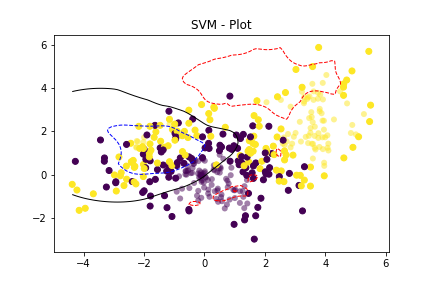
\includegraphics{SVM.png}
\caption{SVM Boundaries}
\end{figure}

\subparagraph{2. ADABOOST}\label{adaboost}

Implementation available from In{[}29{]} onwards

\begin{figure}
\centering
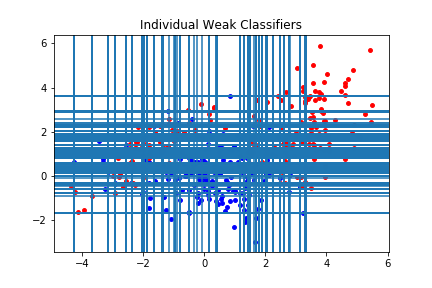
\includegraphics{weak_1075.png}
\caption{Weak Learners}
\end{figure}

\paragraph{DISCUSSION : Observations Comparison among logistic
regression,SVM, neural network, Adaboost for the current dataset. Which
one gives the best results
:}\label{discussion-observations-comparison-among-logistic-regressionsvm-neural-network-adaboost-for-the-current-dataset.-which-one-gives-the-best-results}

Based on the probability of error among all the technique mentioned
above. The probability of error are as follows for all:

\begin{enumerate}
\def\labelenumi{\arabic{enumi}.}
\tightlist
\item
  Logistic Regression : 0.36
\item
  Neural Network : 0.15
\item
  SVM : 0.1375
\item
  Adaboost : 0.1255
\end{enumerate}

\paragraph{OBSERVATIONS}\label{observations}

According to the probability distribution above. Though Adaboost have
the minimum probability of error and the logistic regression has the
maximum probabilty of error. After running the Adaboost algorithm for
about 12000 times it seems there is lot of overfitting. hence if learned
parameters are going to be tested on the test data, here are high
chances that the probability of error is going to be too high, hence
adaboost is not so good for the current data set we are using.

\paragraph{Neural Network}\label{neural-network}

Neural network has the best performance and minimum probability of
error. The weights vectors converges to a constant value faster in case
of Neural Network. While on the same data set in case of SVM and
Adaboost it takes total of around 25-30 minutes and individual 15
minutes for SVM and 10 minutes for ADdaboost, hence we can conclude
Neural Network are much faster and have lower probability of error as
compared to logistic regressiion , SVM , ADABoost and Kmeans.

\section{Code Section}\label{code-section}

    \begin{Verbatim}[commandchars=\\\{\}]
{\color{incolor}In [{\color{incolor}7}]:} \PY{c+c1}{\PYZsh{} \PYZhy{}*\PYZhy{} coding: utf\PYZhy{}8 \PYZhy{}*\PYZhy{}}
        \PY{k+kn}{import} \PY{n+nn}{tensorflow} \PY{k}{as} \PY{n+nn}{tf}
        \PY{k+kn}{import} \PY{n+nn}{numpy} \PY{k}{as} \PY{n+nn}{np}
        \PY{k+kn}{from} \PY{n+nn}{math} \PY{k}{import} \PY{o}{*}
        \PY{k+kn}{import} \PY{n+nn}{matplotlib}\PY{n+nn}{.}\PY{n+nn}{pyplot} \PY{k}{as} \PY{n+nn}{plt}
        \PY{k+kn}{from} \PY{n+nn}{matplotlib} \PY{k}{import} \PY{n}{cm}
        \PY{k+kn}{from} \PY{n+nn}{mpl\PYZus{}toolkits}\PY{n+nn}{.}\PY{n+nn}{mplot3d} \PY{k}{import} \PY{n}{Axes3D}
        \PY{k+kn}{import} \PY{n+nn}{random}
        \PY{k+kn}{from} \PY{n+nn}{scipy}\PY{n+nn}{.}\PY{n+nn}{stats} \PY{k}{import} \PY{n}{norm}
        \PY{k+kn}{from} \PY{n+nn}{IPython}\PY{n+nn}{.}\PY{n+nn}{display} \PY{k}{import} \PY{n}{Image}\PY{p}{,} \PY{n}{display}\PY{p}{,} \PY{n}{Math}\PY{p}{,} \PY{n}{Latex}
        
        \PY{c+c1}{\PYZsh{} Params}
        \PY{n}{total\PYZus{}samples} \PY{o}{=} \PY{l+m+mi}{400}
        \PY{c+c1}{\PYZsh{}HyperParameters }
        \PY{n}{sigma} \PY{o}{=} \PY{l+m+mi}{1} \PY{c+c1}{\PYZsh{} L}
\end{Verbatim}


    \begin{Verbatim}[commandchars=\\\{\}]
{\color{incolor}In [{\color{incolor}8}]:} \PY{c+c1}{\PYZsh{}Class 0}
        \PY{n}{num\PYZus{}samples\PYZus{}0} \PY{o}{=} \PY{n}{total\PYZus{}samples}\PY{o}{/}\PY{l+m+mi}{2}
        
        \PY{c+c1}{\PYZsh{}mean\PYZus{}0 = np.array([0,0]).T \PYZsh{}mean of class 0}
        \PY{n}{mean\PYZus{}0} \PY{o}{=} \PY{p}{(}\PY{l+m+mi}{0}\PY{p}{,}\PY{l+m+mi}{0}\PY{p}{)} \PY{c+c1}{\PYZsh{}mean of class 0}
        
        \PY{c+c1}{\PYZsh{}Eigen Values pair}
        \PY{n}{lambda\PYZus{}01} \PY{o}{=} \PY{l+m+mi}{2}
        \PY{n}{lambda\PYZus{}02} \PY{o}{=} \PY{l+m+mi}{1}
        
        \PY{n}{theta\PYZus{}0} \PY{o}{=} \PY{l+m+mi}{0}
        
        \PY{c+c1}{\PYZsh{} For More info check the http://www.visiondummy.com/2014/04/geometric\PYZhy{}interpretation\PYZhy{}covariance\PYZhy{}matrix/}
        
        \PY{c+c1}{\PYZsh{}Rotation Matrix}
        \PY{n}{q\PYZus{}0} \PY{o}{=} \PY{n}{np}\PY{o}{.}\PY{n}{array}\PY{p}{(}\PY{p}{[}\PY{p}{[}\PY{n}{np}\PY{o}{.}\PY{n}{cos}\PY{p}{(}\PY{n}{theta\PYZus{}0}\PY{p}{)}\PY{p}{,} \PY{o}{\PYZhy{}}\PY{n}{np}\PY{o}{.}\PY{n}{sin}\PY{p}{(}\PY{n}{theta\PYZus{}0}\PY{p}{)}\PY{p}{]}\PY{p}{,}\PY{p}{[}\PY{n}{np}\PY{o}{.}\PY{n}{sin}\PY{p}{(}\PY{n}{theta\PYZus{}0}\PY{p}{)}\PY{p}{,}\PY{n}{np}\PY{o}{.}\PY{n}{cos}\PY{p}{(}\PY{n}{theta\PYZus{}0}\PY{p}{)}\PY{p}{]}\PY{p}{]}\PY{p}{)}
        \PY{n}{q\PYZus{}0\PYZus{}inv} \PY{o}{=} \PY{n}{q\PYZus{}0}\PY{o}{.}\PY{n}{T}
        
        \PY{c+c1}{\PYZsh{} Scaling factor which is represented in Eigen Values Pair}
        \PY{n}{s\PYZus{}0} \PY{o}{=} \PY{n}{np}\PY{o}{.}\PY{n}{array}\PY{p}{(}\PY{p}{[}\PY{p}{[}\PY{n}{lambda\PYZus{}01}\PY{p}{,}\PY{l+m+mi}{0}\PY{p}{]}\PY{p}{,}\PY{p}{[}\PY{l+m+mi}{0}\PY{p}{,}\PY{n}{lambda\PYZus{}02}\PY{p}{]}\PY{p}{]}\PY{p}{)} 
        
        \PY{c+c1}{\PYZsh{}Covariance is computed as the following. }
        
        \PY{n}{cov\PYZus{}0} \PY{o}{=} \PY{n}{q\PYZus{}0}\PY{o}{*}\PY{n}{s\PYZus{}0}\PY{o}{*}\PY{n}{q\PYZus{}0\PYZus{}inv}
        
        \PY{n+nb}{print}\PY{p}{(}\PY{n}{cov\PYZus{}0}\PY{o}{.}\PY{n}{shape}\PY{p}{)}
        
        \PY{c+c1}{\PYZsh{}Multivariate Distribution. samples\PYZus{}0 is the num\PYZus{}samples\PYZus{}0*2D array where each row represent X[1] and x[2] component}
        \PY{n}{samples\PYZus{}0} \PY{o}{=} \PY{n}{np}\PY{o}{.}\PY{n}{random}\PY{o}{.}\PY{n}{multivariate\PYZus{}normal}\PY{p}{(}\PY{n}{mean\PYZus{}0}\PY{p}{,}\PY{n}{cov\PYZus{}0}\PY{p}{,}\PY{n+nb}{int}\PY{p}{(}\PY{n}{num\PYZus{}samples\PYZus{}0}\PY{p}{)}\PY{p}{)}
        
        \PY{c+c1}{\PYZsh{} Data points scaled to zero mean and unit variance.}
        \PY{c+c1}{\PYZsh{}scaled\PYZus{}samples\PYZus{}0 = preprocessing.scale(samples\PYZus{}0)}
        
        \PY{n}{labels\PYZus{}0} \PY{o}{=} \PY{n}{np}\PY{o}{.}\PY{n}{zeros}\PY{p}{(}\PY{p}{(}\PY{n+nb}{int}\PY{p}{(}\PY{n}{num\PYZus{}samples\PYZus{}0}\PY{p}{)}\PY{p}{,}\PY{l+m+mi}{1}\PY{p}{)}\PY{p}{)} \PY{c+c1}{\PYZsh{} label for class 0 as \PYZhy{}1}
        \PY{n}{labels\PYZus{}0}\PY{p}{[}\PY{p}{:}\PY{p}{,}\PY{l+m+mi}{0}\PY{p}{]} \PY{o}{=} \PY{o}{\PYZhy{}}\PY{l+m+mi}{1}
        
        \PY{c+c1}{\PYZsh{} Formation of the whole data set with it\PYZsq{}s corresponding labels}
        \PY{n}{sample\PYZus{}0\PYZus{}data\PYZus{}set} \PY{o}{=} \PY{n}{np}\PY{o}{.}\PY{n}{concatenate}\PY{p}{(}\PY{p}{(}\PY{n}{samples\PYZus{}0}\PY{p}{,} \PY{n}{labels\PYZus{}0}\PY{p}{)}\PY{p}{,}\PY{n}{axis} \PY{o}{=} \PY{l+m+mi}{1}\PY{p}{)}
        \PY{c+c1}{\PYZsh{}scaled\PYZus{}sample\PYZus{}0\PYZus{}data\PYZus{}set = np.concatenate((scaled\PYZus{}samples\PYZus{}0, labels\PYZus{}0),axis = 1)}
        
        \PY{c+c1}{\PYZsh{}Class 1 Gaussian Mixture with two components}
        
        \PY{n}{num\PYZus{}samples\PYZus{}1} \PY{o}{=} \PY{n}{total\PYZus{}samples}\PY{o}{/}\PY{l+m+mi}{2}
        \PY{n}{pi\PYZus{}A} \PY{o}{=} \PY{l+m+mi}{1}\PY{o}{/}\PY{l+m+mf}{3.0}
        \PY{n}{pi\PYZus{}B} \PY{o}{=} \PY{l+m+mi}{2}\PY{o}{/}\PY{l+m+mf}{3.0}
        \PY{c+c1}{\PYZsh{}\PYZsh{}\PYZsh{}\PYZsh{}\PYZsh{}\PYZsh{} Start of Component A}
        \PY{c+c1}{\PYZsh{}\PYZsh{} Component A}
        
        \PY{n}{num\PYZus{}samples\PYZus{}1A} \PY{o}{=} \PY{n}{np}\PY{o}{.}\PY{n}{random}\PY{o}{.}\PY{n}{binomial}\PY{p}{(}\PY{n}{num\PYZus{}samples\PYZus{}1}\PY{p}{,}\PY{n}{pi\PYZus{}A}\PY{p}{)}
        \PY{n}{num\PYZus{}samples\PYZus{}1B} \PY{o}{=} \PY{n}{num\PYZus{}samples\PYZus{}1} \PY{o}{\PYZhy{}} \PY{n}{num\PYZus{}samples\PYZus{}1A}
        
        \PY{n}{mean\PYZus{}1A} \PY{o}{=} \PY{n}{np}\PY{o}{.}\PY{n}{array}\PY{p}{(}\PY{p}{[}\PY{o}{\PYZhy{}}\PY{l+m+mi}{2}\PY{p}{,}\PY{l+m+mi}{1}\PY{p}{]}\PY{p}{)}\PY{o}{.}\PY{n}{T} \PY{c+c1}{\PYZsh{}mean of class 1 component A}
        
        \PY{c+c1}{\PYZsh{}Eigen Values pair}
        \PY{n}{lambda\PYZus{}1A1} \PY{o}{=} \PY{l+m+mi}{2}
        \PY{n}{lambda\PYZus{}1A2} \PY{o}{=} \PY{l+m+mi}{1}\PY{o}{/}\PY{l+m+mf}{4.0}
        
        \PY{n}{theta\PYZus{}1A} \PY{o}{=} \PY{o}{\PYZhy{}}\PY{l+m+mi}{3}\PY{o}{*}\PY{n}{np}\PY{o}{.}\PY{n}{pi}\PY{o}{/}\PY{l+m+mf}{4.0}
        
        \PY{c+c1}{\PYZsh{} For More info check the http://www.visiondummy.com/2014/04/geometric\PYZhy{}interpretation\PYZhy{}covariance\PYZhy{}matrix/}
        
        \PY{c+c1}{\PYZsh{}Rotation Matrix}
        \PY{n}{q\PYZus{}1A} \PY{o}{=} \PY{n}{np}\PY{o}{.}\PY{n}{array}\PY{p}{(}\PY{p}{[}\PY{p}{[}\PY{n}{np}\PY{o}{.}\PY{n}{cos}\PY{p}{(}\PY{n}{theta\PYZus{}1A}\PY{p}{)}\PY{p}{,} \PY{o}{\PYZhy{}}\PY{n}{np}\PY{o}{.}\PY{n}{sin}\PY{p}{(}\PY{n}{theta\PYZus{}1A}\PY{p}{)}\PY{p}{]}\PY{p}{,}\PY{p}{[}\PY{n}{np}\PY{o}{.}\PY{n}{sin}\PY{p}{(}\PY{n}{theta\PYZus{}1A}\PY{p}{)}\PY{p}{,}\PY{n}{np}\PY{o}{.}\PY{n}{cos}\PY{p}{(}\PY{n}{theta\PYZus{}1A}\PY{p}{)}\PY{p}{]}\PY{p}{]}\PY{p}{)}
        \PY{n}{q\PYZus{}1A\PYZus{}inv} \PY{o}{=} \PY{n}{q\PYZus{}1A}\PY{o}{.}\PY{n}{T}
        
        \PY{c+c1}{\PYZsh{} Scaling factor which is represented in Eigen Values Pair}
        \PY{n}{s\PYZus{}1A} \PY{o}{=} \PY{n}{np}\PY{o}{.}\PY{n}{array}\PY{p}{(}\PY{p}{[}\PY{p}{[}\PY{n}{lambda\PYZus{}1A1}\PY{p}{,}\PY{l+m+mi}{0}\PY{p}{]}\PY{p}{,}\PY{p}{[}\PY{l+m+mi}{0}\PY{p}{,}\PY{n}{lambda\PYZus{}1A2}\PY{p}{]}\PY{p}{]}\PY{p}{)} 
        
        \PY{c+c1}{\PYZsh{}Covariance is computed as the following. }
        \PY{n}{cov\PYZus{}1A} \PY{o}{=} \PY{n}{q\PYZus{}1A}\PY{o}{.}\PY{n}{dot}\PY{p}{(}\PY{n}{s\PYZus{}1A}\PY{p}{)}\PY{o}{.}\PY{n}{dot}\PY{p}{(}\PY{n}{q\PYZus{}1A\PYZus{}inv}\PY{p}{)}
        
        
        \PY{c+c1}{\PYZsh{}Multivariate Distribution. samples\PYZus{}0 is the num\PYZus{}samples\PYZus{}0*2D array where each row represent X[1] and x[2] component}
        \PY{n}{samples\PYZus{}1A} \PY{o}{=} \PY{n}{np}\PY{o}{.}\PY{n}{random}\PY{o}{.}\PY{n}{multivariate\PYZus{}normal}\PY{p}{(}\PY{n}{mean\PYZus{}1A}\PY{p}{,}\PY{n}{cov\PYZus{}1A}\PY{p}{,}\PY{n}{num\PYZus{}samples\PYZus{}1A}\PY{p}{)}
        
        \PY{c+c1}{\PYZsh{} Data points scaled to zero mean and unit variance.}
        \PY{c+c1}{\PYZsh{}scaled\PYZus{}samples\PYZus{}1A = preprocessing.scale(samples\PYZus{}1A)}
        
        \PY{c+c1}{\PYZsh{}\PYZsh{}\PYZsh{}\PYZsh{}\PYZsh{}\PYZsh{} End of Component A}
        
        \PY{c+c1}{\PYZsh{}\PYZsh{}\PYZsh{}\PYZsh{}\PYZsh{}\PYZsh{} Start of Component B}
        \PY{c+c1}{\PYZsh{}\PYZsh{} Component B}
        
        \PY{n}{mean\PYZus{}1B} \PY{o}{=} \PY{n}{np}\PY{o}{.}\PY{n}{array}\PY{p}{(}\PY{p}{[}\PY{l+m+mi}{3}\PY{p}{,}\PY{l+m+mi}{2}\PY{p}{]}\PY{p}{)}\PY{o}{.}\PY{n}{T} \PY{c+c1}{\PYZsh{}mean of class 1 component A}
        
        \PY{c+c1}{\PYZsh{}Eigen Values pair}
        \PY{n}{lambda\PYZus{}1B1} \PY{o}{=} \PY{l+m+mi}{3}
        \PY{n}{lambda\PYZus{}1B2} \PY{o}{=} \PY{l+m+mi}{1}
        
        \PY{n}{theta\PYZus{}1B} \PY{o}{=} \PY{n}{np}\PY{o}{.}\PY{n}{pi}\PY{o}{/}\PY{l+m+mf}{4.0}
        
        \PY{c+c1}{\PYZsh{} For More info check the http://www.visiondummy.com/2014/04/geometric\PYZhy{}interpretation\PYZhy{}covariance\PYZhy{}matrix/}
        
        \PY{c+c1}{\PYZsh{}Rotation Matrix}
        \PY{n}{q\PYZus{}1B} \PY{o}{=} \PY{n}{np}\PY{o}{.}\PY{n}{array}\PY{p}{(}\PY{p}{[}\PY{p}{[}\PY{n}{np}\PY{o}{.}\PY{n}{cos}\PY{p}{(}\PY{n}{theta\PYZus{}1B}\PY{p}{)}\PY{p}{,} \PY{o}{\PYZhy{}}\PY{n}{np}\PY{o}{.}\PY{n}{sin}\PY{p}{(}\PY{n}{theta\PYZus{}1B}\PY{p}{)}\PY{p}{]}\PY{p}{,}\PY{p}{[}\PY{n}{np}\PY{o}{.}\PY{n}{sin}\PY{p}{(}\PY{n}{theta\PYZus{}1B}\PY{p}{)}\PY{p}{,}\PY{n}{np}\PY{o}{.}\PY{n}{cos}\PY{p}{(}\PY{n}{theta\PYZus{}1B}\PY{p}{)}\PY{p}{]}\PY{p}{]}\PY{p}{)}
        \PY{n}{q\PYZus{}1B\PYZus{}inv} \PY{o}{=} \PY{n}{q\PYZus{}1B}\PY{o}{.}\PY{n}{T}
        
        \PY{c+c1}{\PYZsh{} Scaling factor which is represented in Eigen Values Pair}
        \PY{n}{s\PYZus{}1B} \PY{o}{=} \PY{n}{np}\PY{o}{.}\PY{n}{array}\PY{p}{(}\PY{p}{[}\PY{p}{[}\PY{n}{lambda\PYZus{}1B1}\PY{p}{,}\PY{l+m+mi}{0}\PY{p}{]}\PY{p}{,}\PY{p}{[}\PY{l+m+mi}{0}\PY{p}{,}\PY{n}{lambda\PYZus{}1B2}\PY{p}{]}\PY{p}{]}\PY{p}{)} 
        
        \PY{c+c1}{\PYZsh{}Covariance is computed as the following. }
        
        \PY{n}{cov\PYZus{}1B} \PY{o}{=} \PY{n}{q\PYZus{}1B}\PY{o}{.}\PY{n}{dot}\PY{p}{(}\PY{n}{s\PYZus{}1B}\PY{p}{)}\PY{o}{.}\PY{n}{dot}\PY{p}{(}\PY{n}{q\PYZus{}1B\PYZus{}inv}\PY{p}{)}
        
        \PY{c+c1}{\PYZsh{}Multivariate Distribution. samples\PYZus{}0 is the num\PYZus{}samples\PYZus{}0*2D array where each row represent X[1] and x[2] component}
        \PY{n}{samples\PYZus{}1B} \PY{o}{=} \PY{n}{np}\PY{o}{.}\PY{n}{random}\PY{o}{.}\PY{n}{multivariate\PYZus{}normal}\PY{p}{(}\PY{n}{mean\PYZus{}1B}\PY{p}{,}\PY{n}{cov\PYZus{}1B}\PY{p}{,}\PY{n+nb}{int}\PY{p}{(}\PY{n}{num\PYZus{}samples\PYZus{}1B}\PY{p}{)}\PY{p}{)}
        
        \PY{c+c1}{\PYZsh{} Data points scaled to zero mean and unit variance.}
        \PY{c+c1}{\PYZsh{}scaled\PYZus{}samples\PYZus{}1B = preprocessing.scale(samples\PYZus{}1B)}
        
        \PY{c+c1}{\PYZsh{}\PYZsh{}\PYZsh{}\PYZsh{}\PYZsh{}\PYZsh{} End of Component B}
        \PY{n}{samples\PYZus{}1} \PY{o}{=} \PY{n}{np}\PY{o}{.}\PY{n}{concatenate}\PY{p}{(}\PY{p}{(}\PY{n}{samples\PYZus{}1A}\PY{p}{,}\PY{n}{samples\PYZus{}1B}\PY{p}{)}\PY{p}{)}
        \PY{c+c1}{\PYZsh{}samples\PYZus{}1 = pi\PYZus{}A*samples\PYZus{}1A + pi\PYZus{}B*samples\PYZus{}1B}
        \PY{c+c1}{\PYZsh{}scaled\PYZus{}samples\PYZus{}1 = pi\PYZus{}A*scaled\PYZus{}samples\PYZus{}1A + pi\PYZus{}B*scaled\PYZus{}samples\PYZus{}1B}
        
        \PY{n}{labels\PYZus{}1} \PY{o}{=} \PY{n}{np}\PY{o}{.}\PY{n}{ones}\PY{p}{(}\PY{p}{(}\PY{n+nb}{int}\PY{p}{(}\PY{n}{num\PYZus{}samples\PYZus{}1}\PY{p}{)}\PY{p}{,}\PY{l+m+mi}{1}\PY{p}{)}\PY{p}{)} \PY{c+c1}{\PYZsh{} label for class 1 as +1}
        \PY{c+c1}{\PYZsh{}labels\PYZus{}1[:,0] = 1}
        
        \PY{c+c1}{\PYZsh{} Formation of the whole data set with it\PYZsq{}s corresponding labels}
        \PY{n}{sample\PYZus{}1\PYZus{}data\PYZus{}set} \PY{o}{=} \PY{n}{np}\PY{o}{.}\PY{n}{concatenate}\PY{p}{(}\PY{p}{(}\PY{n}{samples\PYZus{}1}\PY{p}{,} \PY{n}{labels\PYZus{}1}\PY{p}{)}\PY{p}{,}\PY{n}{axis} \PY{o}{=} \PY{l+m+mi}{1}\PY{p}{)}
        \PY{c+c1}{\PYZsh{}scaled\PYZus{}sample\PYZus{}1\PYZus{}data\PYZus{}set = np.concatenate((scaled\PYZus{}samples\PYZus{}1, labels\PYZus{}0),axis = 1)}
\end{Verbatim}


    \begin{Verbatim}[commandchars=\\\{\}]
(2, 2)

    \end{Verbatim}

    \begin{Verbatim}[commandchars=\\\{\}]
{\color{incolor}In [{\color{incolor}9}]:} \PY{c+c1}{\PYZsh{} plot samples from Class 0 (X\PYZus{}0) and Class 1 (X\PYZus{}1) plt.figure(0)}
        \PY{c+c1}{\PYZsh{}maxX = 7.5 \PYZsh{} region to plot}
        \PY{c+c1}{\PYZsh{}maxY = 7.5}
        \PY{n}{plt}\PY{o}{.}\PY{n}{title}\PY{p}{(}\PY{l+s+s2}{\PYZdq{}}\PY{l+s+s2}{Distribution of the Data}\PY{l+s+s2}{\PYZdq{}}\PY{p}{)}
        \PY{n}{plt}\PY{o}{.}\PY{n}{scatter}\PY{p}{(}\PY{n}{sample\PYZus{}0\PYZus{}data\PYZus{}set}\PY{p}{[}\PY{p}{:}\PY{p}{,}\PY{l+m+mi}{0}\PY{p}{]}\PY{p}{,} \PY{n}{sample\PYZus{}0\PYZus{}data\PYZus{}set}\PY{p}{[}\PY{p}{:}\PY{p}{,}\PY{l+m+mi}{1}\PY{p}{]}\PY{p}{,} \PY{n}{s}\PY{o}{=}\PY{l+m+mi}{15}\PY{p}{,} \PY{n}{c}\PY{o}{=}\PY{l+s+s2}{\PYZdq{}}\PY{l+s+s2}{blue}\PY{l+s+s2}{\PYZdq{}}\PY{p}{)} 
        \PY{n}{plt}\PY{o}{.}\PY{n}{scatter}\PY{p}{(}\PY{n}{sample\PYZus{}1\PYZus{}data\PYZus{}set}\PY{p}{[}\PY{p}{:}\PY{p}{,}\PY{l+m+mi}{0}\PY{p}{]}\PY{p}{,} \PY{n}{sample\PYZus{}1\PYZus{}data\PYZus{}set}\PY{p}{[}\PY{p}{:}\PY{p}{,}\PY{l+m+mi}{1}\PY{p}{]}\PY{p}{,} \PY{n}{s}\PY{o}{=}\PY{l+m+mi}{15}\PY{p}{,} \PY{n}{c}\PY{o}{=}\PY{l+s+s2}{\PYZdq{}}\PY{l+s+s2}{red}\PY{l+s+s2}{\PYZdq{}}\PY{p}{)} 
        \PY{c+c1}{\PYZsh{}plt.axis([\PYZhy{}maxX, maxX, \PYZhy{}maxY, maxY])}
        \PY{n}{plt}\PY{o}{.}\PY{n}{show}\PY{p}{(}\PY{p}{)}
\end{Verbatim}


    \begin{center}
    \adjustimage{max size={0.9\linewidth}{0.9\paperheight}}{output_3_0.png}
    \end{center}
    { \hspace*{\fill} \\}
    
    \begin{Verbatim}[commandchars=\\\{\}]
{\color{incolor}In [{\color{incolor}10}]:} \PY{n}{data\PYZus{}set} \PY{o}{=} \PY{n}{np}\PY{o}{.}\PY{n}{concatenate}\PY{p}{(}\PY{p}{(}\PY{n}{sample\PYZus{}0\PYZus{}data\PYZus{}set}\PY{p}{,}\PY{n}{sample\PYZus{}1\PYZus{}data\PYZus{}set}\PY{p}{)}\PY{p}{)}
         \PY{n}{np}\PY{o}{.}\PY{n}{random}\PY{o}{.}\PY{n}{shuffle}\PY{p}{(}\PY{n}{data\PYZus{}set}\PY{p}{)}
         \PY{n}{data\PYZus{}set}
\end{Verbatim}


\begin{Verbatim}[commandchars=\\\{\}]
{\color{outcolor}Out[{\color{outcolor}10}]:} array([[-0.91828172, -0.77850471, -1.        ],
                [ 0.0321756 , -0.1082165 , -1.        ],
                [ 0.83151929, -1.1431078 , -1.        ],
                {\ldots},
                [-2.1412134 ,  1.21831522,  1.        ],
                [ 1.64712048, -2.96929057, -1.        ],
                [-0.36585517,  0.49704773, -1.        ]])
\end{Verbatim}
            
    \subsection{1. SVM:}\label{svm}

\subsubsection{Gaussian kernel k(x, x') = exp (− (\textbar{}\textbar{}x
− x'\textbar{}\textbar{}\^{}2) / 2 *
(L\^{}2)}\label{gaussian-kernel-kx-x-exp-x-x2-2-l2}

1.1) Plot the decision boundaries, and display the support vectors.

    \begin{Verbatim}[commandchars=\\\{\}]
{\color{incolor}In [{\color{incolor}11}]:} \PY{k}{def} \PY{n+nf}{gaussian\PYZus{}kernel}\PY{p}{(}\PY{n}{x}\PY{p}{,} \PY{n}{y}\PY{p}{,} \PY{n}{sigma}\PY{o}{=}\PY{l+m+mf}{0.9}\PY{p}{)}\PY{p}{:}
             \PY{k}{if} \PY{n}{np}\PY{o}{.}\PY{n}{ndim}\PY{p}{(}\PY{n}{x}\PY{p}{)} \PY{o}{==} \PY{l+m+mi}{1} \PY{o+ow}{and} \PY{n}{np}\PY{o}{.}\PY{n}{ndim}\PY{p}{(}\PY{n}{y}\PY{p}{)} \PY{o}{==} \PY{l+m+mi}{1}\PY{p}{:}
                 \PY{n}{result} \PY{o}{=} \PY{n}{np}\PY{o}{.}\PY{n}{exp}\PY{p}{(}\PY{o}{\PYZhy{}} \PY{n}{np}\PY{o}{.}\PY{n}{linalg}\PY{o}{.}\PY{n}{norm}\PY{p}{(}\PY{n}{x} \PY{o}{\PYZhy{}} \PY{n}{y}\PY{p}{)} \PY{o}{/} \PY{p}{(}\PY{l+m+mi}{2} \PY{o}{*} \PY{n}{sigma} \PY{o}{*}\PY{o}{*} \PY{l+m+mi}{2}\PY{p}{)}\PY{p}{)}
             \PY{k}{elif} \PY{p}{(}\PY{n}{np}\PY{o}{.}\PY{n}{ndim}\PY{p}{(}\PY{n}{x}\PY{p}{)} \PY{o}{\PYZgt{}} \PY{l+m+mi}{1} \PY{o+ow}{and} \PY{n}{np}\PY{o}{.}\PY{n}{ndim}\PY{p}{(}\PY{n}{y}\PY{p}{)} \PY{o}{==} \PY{l+m+mi}{1}\PY{p}{)} \PY{o+ow}{or} \PY{p}{(}\PY{n}{np}\PY{o}{.}\PY{n}{ndim}\PY{p}{(}\PY{n}{x}\PY{p}{)} \PY{o}{==} \PY{l+m+mi}{1} \PY{o+ow}{and} \PY{n}{np}\PY{o}{.}\PY{n}{ndim}\PY{p}{(}\PY{n}{y}\PY{p}{)} \PY{o}{\PYZgt{}} \PY{l+m+mi}{1}\PY{p}{)}\PY{p}{:}
                 \PY{n}{result} \PY{o}{=} \PY{n}{np}\PY{o}{.}\PY{n}{exp}\PY{p}{(}\PY{o}{\PYZhy{}} \PY{n}{np}\PY{o}{.}\PY{n}{linalg}\PY{o}{.}\PY{n}{norm}\PY{p}{(}\PY{n}{x} \PY{o}{\PYZhy{}} \PY{n}{y}\PY{p}{,} \PY{n}{axis}\PY{o}{=}\PY{l+m+mi}{1}\PY{p}{)} \PY{o}{/} \PY{p}{(}\PY{l+m+mi}{2} \PY{o}{*} \PY{n}{sigma} \PY{o}{*}\PY{o}{*} \PY{l+m+mi}{2}\PY{p}{)}\PY{p}{)}
             \PY{k}{elif} \PY{n}{np}\PY{o}{.}\PY{n}{ndim}\PY{p}{(}\PY{n}{x}\PY{p}{)} \PY{o}{\PYZgt{}} \PY{l+m+mi}{1} \PY{o+ow}{and} \PY{n}{np}\PY{o}{.}\PY{n}{ndim}\PY{p}{(}\PY{n}{y}\PY{p}{)} \PY{o}{\PYZgt{}} \PY{l+m+mi}{1}\PY{p}{:}
                 \PY{n}{result} \PY{o}{=} \PY{n}{np}\PY{o}{.}\PY{n}{exp}\PY{p}{(}\PY{o}{\PYZhy{}} \PY{n}{np}\PY{o}{.}\PY{n}{linalg}\PY{o}{.}\PY{n}{norm}\PY{p}{(}\PY{n}{x}\PY{p}{[}\PY{p}{:}\PY{p}{,} \PY{n}{np}\PY{o}{.}\PY{n}{newaxis}\PY{p}{]} \PY{o}{\PYZhy{}} \PY{n}{y}\PY{p}{[}\PY{n}{np}\PY{o}{.}\PY{n}{newaxis}\PY{p}{,} \PY{p}{:}\PY{p}{]}\PY{p}{,} \PY{n}{axis}\PY{o}{=}\PY{l+m+mi}{2}\PY{p}{)} \PY{o}{/} \PY{p}{(}\PY{l+m+mi}{2} \PY{o}{*} \PY{n}{sigma} \PY{o}{*}\PY{o}{*} \PY{l+m+mi}{2}\PY{p}{)}\PY{p}{)}
             \PY{k}{return} \PY{n}{result}
         
         \PY{c+c1}{\PYZsh{}x\PYZus{}len, y\PYZus{}len = 5, 10}
         \PY{c+c1}{\PYZsh{}gaussian\PYZus{}kernel(np.random.rand(x\PYZus{}len, 1), np.random.rand(y\PYZus{}len, 1)).shape == (5,10)}
         
         \PY{c+c1}{\PYZsh{} Objective function to optimize\PYZsh{} Objec }
         \PY{k}{def} \PY{n+nf}{objective\PYZus{}function}\PY{p}{(}\PY{n}{alphas}\PY{p}{,}\PY{n}{kernel}\PY{p}{,} \PY{n}{data}\PY{p}{)}\PY{p}{:}
             \PY{l+s+sd}{\PYZdq{}\PYZdq{}\PYZdq{}Returns the SVM objective function based in the input model defined by:}
         \PY{l+s+sd}{    `alphas`: vector of Lagrange multipliers}
         \PY{l+s+sd}{    `target`: vector of class labels (\PYZhy{}1 or 1) for training data}
         \PY{l+s+sd}{    `kernel`: kernel function}
         \PY{l+s+sd}{    `X\PYZus{}train`: training data for model.\PYZdq{}\PYZdq{}\PYZdq{}}
             \PY{k}{return} \PY{n}{np}\PY{o}{.}\PY{n}{sum}\PY{p}{(}\PY{n}{alphas}\PY{p}{)} \PY{o}{\PYZhy{}} \PY{l+m+mf}{0.5}\PY{o}{*} \PY{n}{np}\PY{o}{.}\PY{n}{sum}\PY{p}{(}\PY{n}{data}\PY{p}{[}\PY{p}{:}\PY{p}{,}\PY{l+m+mi}{2}\PY{p}{]} \PY{o}{*} \PY{n}{data}\PY{p}{[}\PY{p}{:}\PY{p}{,}\PY{l+m+mi}{2}\PY{p}{]} \PY{o}{*} \PY{n}{gaussian\PYZus{}kernel}\PY{p}{(}\PY{n}{data}\PY{p}{[}\PY{p}{:}\PY{p}{,}\PY{l+m+mi}{0}\PY{p}{:}\PY{l+m+mi}{2}\PY{p}{]}\PY{p}{,} \PY{n}{data}\PY{p}{[}\PY{p}{:}\PY{p}{,}\PY{l+m+mi}{0}\PY{p}{:}\PY{l+m+mi}{2}\PY{p}{]}\PY{p}{)} \PY{o}{*} \PY{n}{aplhas} \PY{o}{*} \PY{n}{aplhas}\PY{p}{)}
         
         
         \PY{c+c1}{\PYZsh{} Decision function}
         \PY{k}{def} \PY{n+nf}{decision\PYZus{}function}\PY{p}{(}\PY{n}{alphas}\PY{p}{,}\PY{n}{data}\PY{p}{,}\PY{n}{b}\PY{p}{,}\PY{n}{X\PYZus{}Test}\PY{p}{)}\PY{p}{:}
             \PY{l+s+sd}{\PYZdq{}\PYZdq{}\PYZdq{}Applies the SVM decision function to the input feature vectors in `x\PYZus{}test`.\PYZdq{}\PYZdq{}\PYZdq{}}
             \PY{c+c1}{\PYZsh{} The following is the loop function.}
             \PY{n+nb}{sum} \PY{o}{=} \PY{l+m+mi}{0}
             \PY{k}{for} \PY{n}{i} \PY{o+ow}{in} \PY{n+nb}{range}\PY{p}{(}\PY{n+nb}{len}\PY{p}{(}\PY{n}{data}\PY{p}{)}\PY{p}{)}\PY{p}{:}
                 \PY{n+nb}{sum} \PY{o}{+}\PY{o}{=} \PY{n}{alphas}\PY{p}{[}\PY{n}{i}\PY{p}{]} \PY{o}{*} \PY{n}{data}\PY{p}{[}\PY{n}{i}\PY{p}{,}\PY{l+m+mi}{2}\PY{p}{]} \PY{o}{*} \PY{n}{gaussian\PYZus{}kernel}\PY{p}{(}\PY{n}{data}\PY{p}{[}\PY{n}{i}\PY{p}{,}\PY{l+m+mi}{0}\PY{p}{:}\PY{l+m+mi}{2}\PY{p}{]}\PY{p}{,}\PY{n}{X\PYZus{}Test}\PY{p}{)}
             \PY{n}{f\PYZus{}x} \PY{o}{=} \PY{n+nb}{sum} \PY{o}{+} \PY{n}{b}
             \PY{k}{return} \PY{n}{f\PYZus{}x}
         
         \PY{k}{def} \PY{n+nf}{compute\PYZus{}range}\PY{p}{(}\PY{n}{alphas}\PY{p}{,}\PY{n}{i}\PY{p}{,}\PY{n}{j}\PY{p}{,}\PY{n}{data}\PY{p}{,}\PY{n}{C}\PY{p}{)}\PY{p}{:}
             \PY{k}{if} \PY{p}{(}\PY{n}{data}\PY{p}{[}\PY{n}{i}\PY{p}{,}\PY{l+m+mi}{2}\PY{p}{]} \PY{o}{!=} \PY{n}{data}\PY{p}{[}\PY{n}{j}\PY{p}{,}\PY{l+m+mi}{2}\PY{p}{]}\PY{p}{)}\PY{p}{:}
                 \PY{n}{L} \PY{o}{=} \PY{n+nb}{max}\PY{p}{(}\PY{l+m+mi}{0}\PY{p}{,}\PY{n}{alphas}\PY{p}{[}\PY{n}{j}\PY{p}{]}\PY{o}{\PYZhy{}}\PY{n}{alphas}\PY{p}{[}\PY{n}{i}\PY{p}{]}\PY{p}{)}
                 \PY{n}{H} \PY{o}{=} \PY{n+nb}{min}\PY{p}{(}\PY{n}{C}\PY{p}{,}\PY{n}{C}\PY{o}{+}\PY{n}{alphas}\PY{p}{[}\PY{n}{j}\PY{p}{]}\PY{o}{\PYZhy{}}\PY{n}{alphas}\PY{p}{[}\PY{n}{i}\PY{p}{]}\PY{p}{)}
             \PY{k}{elif} \PY{p}{(}\PY{n}{data}\PY{p}{[}\PY{n}{i}\PY{p}{,}\PY{l+m+mi}{2}\PY{p}{]} \PY{o}{==} \PY{n}{data}\PY{p}{[}\PY{n}{j}\PY{p}{,}\PY{l+m+mi}{2}\PY{p}{]}\PY{p}{)}\PY{p}{:}  
                 \PY{n}{L} \PY{o}{=} \PY{n+nb}{max}\PY{p}{(}\PY{l+m+mi}{0}\PY{p}{,}\PY{n}{alphas}\PY{p}{[}\PY{n}{i}\PY{p}{]}\PY{o}{+}\PY{n}{alphas}\PY{p}{[}\PY{n}{j}\PY{p}{]}\PY{o}{\PYZhy{}}\PY{n}{C}\PY{p}{)}
                 \PY{n}{H} \PY{o}{=} \PY{n+nb}{min}\PY{p}{(}\PY{n}{C}\PY{p}{,}\PY{n}{alphas}\PY{p}{[}\PY{n}{i}\PY{p}{]}\PY{o}{+}\PY{n}{alphas}\PY{p}{[}\PY{n}{j}\PY{p}{]}\PY{p}{)}
             \PY{k}{return} \PY{n}{L}\PY{p}{,}\PY{n}{H}    
         
         \PY{c+c1}{\PYZsh{} Intialization}
         \PY{n}{alphas} \PY{o}{=} \PY{n}{np}\PY{o}{.}\PY{n}{zeros}\PY{p}{(}\PY{n+nb}{len}\PY{p}{(}\PY{n}{data\PYZus{}set}\PY{p}{)}\PY{p}{)}
         \PY{n}{b} \PY{o}{=} \PY{l+m+mf}{0.0}
         \PY{n}{passes} \PY{o}{=} \PY{l+m+mi}{0}
         \PY{n}{max\PYZus{}passes} \PY{o}{=} \PY{l+m+mi}{300}
         \PY{n}{C} \PY{o}{=} \PY{l+m+mf}{0.2}
         \PY{n}{tol} \PY{o}{=} \PY{l+m+mf}{0.001}
         \PY{n}{m} \PY{o}{=} \PY{n+nb}{len}\PY{p}{(}\PY{n}{data\PYZus{}set}\PY{p}{)}
         \PY{n}{data} \PY{o}{=} \PY{n}{data\PYZus{}set}
         
         \PY{k}{while}\PY{p}{(}\PY{n}{passes} \PY{o}{\PYZlt{}} \PY{n}{max\PYZus{}passes}\PY{p}{)}\PY{p}{:}
             
             \PY{n}{num\PYZus{}changed\PYZus{}alphas} \PY{o}{=} \PY{l+m+mi}{0}
             \PY{k}{for} \PY{n}{i} \PY{o+ow}{in} \PY{n+nb}{range}\PY{p}{(}\PY{n}{m}\PY{p}{)}\PY{p}{:}
                 \PY{n}{E\PYZus{}i} \PY{o}{=} \PY{n}{decision\PYZus{}function}\PY{p}{(}\PY{n}{alphas}\PY{p}{,}\PY{n}{data}\PY{p}{,}\PY{n}{b}\PY{p}{,}\PY{n}{data}\PY{p}{[}\PY{n}{i}\PY{p}{,}\PY{l+m+mi}{0}\PY{p}{:}\PY{l+m+mi}{2}\PY{p}{]}\PY{p}{)} \PY{o}{\PYZhy{}} \PY{n}{data}\PY{p}{[}\PY{n}{i}\PY{p}{,}\PY{l+m+mi}{2}\PY{p}{]}
                 \PY{k}{if}\PY{p}{(}\PY{p}{(}\PY{p}{(}\PY{n}{data}\PY{p}{[}\PY{n}{i}\PY{p}{,}\PY{l+m+mi}{2}\PY{p}{]} \PY{o}{*} \PY{n}{E\PYZus{}i}\PY{p}{)} \PY{o}{\PYZlt{}} \PY{p}{(}\PY{o}{\PYZhy{}}\PY{l+m+mi}{1}\PY{p}{)} \PY{o}{*} \PY{n}{tol} \PY{o+ow}{and} \PY{n}{alphas}\PY{p}{[}\PY{n}{i}\PY{p}{]} \PY{o}{\PYZlt{}} \PY{n}{C}\PY{p}{)} \PY{o+ow}{or} \PY{p}{(}\PY{p}{(}\PY{n}{data}\PY{p}{[}\PY{n}{i}\PY{p}{,}\PY{l+m+mi}{2}\PY{p}{]}\PY{o}{*}\PY{n}{E\PYZus{}i}\PY{p}{)}\PY{o}{\PYZgt{}}\PY{n}{tol} \PY{o+ow}{and} \PY{n}{alphas}\PY{p}{[}\PY{n}{i}\PY{p}{]}\PY{o}{\PYZgt{}}\PY{l+m+mi}{0} \PY{p}{)}\PY{p}{)}\PY{p}{:}
                     \PY{n}{j} \PY{o}{=} \PY{n}{np}\PY{o}{.}\PY{n}{random}\PY{o}{.}\PY{n}{randint}\PY{p}{(}\PY{l+m+mi}{0}\PY{p}{,}\PY{n}{m}\PY{p}{)}
                     \PY{k}{while}\PY{p}{(}\PY{n}{j}\PY{o}{==}\PY{n}{i}\PY{p}{)}\PY{p}{:}
                         \PY{n}{j} \PY{o}{=} \PY{n}{np}\PY{o}{.}\PY{n}{random}\PY{o}{.}\PY{n}{randint}\PY{p}{(}\PY{l+m+mi}{0}\PY{p}{,}\PY{n}{m}\PY{p}{)}
                     
                     \PY{n}{E\PYZus{}j} \PY{o}{=} \PY{n}{decision\PYZus{}function}\PY{p}{(}\PY{n}{alphas}\PY{p}{,}\PY{n}{data}\PY{p}{,}\PY{n}{b}\PY{p}{,}\PY{n}{data}\PY{p}{[}\PY{n}{j}\PY{p}{,}\PY{l+m+mi}{0}\PY{p}{:}\PY{l+m+mi}{2}\PY{p}{]}\PY{p}{)} \PY{o}{\PYZhy{}} \PY{n}{data}\PY{p}{[}\PY{n}{j}\PY{p}{,}\PY{l+m+mi}{2}\PY{p}{]}
         
                     \PY{n}{alpha\PYZus{}i\PYZus{}old} \PY{o}{=} \PY{n}{alphas}\PY{p}{[}\PY{n}{i}\PY{p}{]}
                     \PY{n}{alpha\PYZus{}j\PYZus{}old} \PY{o}{=} \PY{n}{alphas}\PY{p}{[}\PY{n}{j}\PY{p}{]}
                     
                     \PY{n}{L}\PY{p}{,}\PY{n}{H} \PY{o}{=} \PY{n}{compute\PYZus{}range}\PY{p}{(}\PY{n}{alphas}\PY{p}{,}\PY{n}{i}\PY{p}{,}\PY{n}{j}\PY{p}{,}\PY{n}{data}\PY{p}{,}\PY{n}{C}\PY{p}{)}
                     
                     \PY{k}{if} \PY{n}{L} \PY{o}{==} \PY{n}{H}\PY{p}{:}
                         \PY{k}{continue}
                     \PY{n}{k\PYZus{}ij} \PY{o}{=} \PY{n}{gaussian\PYZus{}kernel}\PY{p}{(}\PY{n}{data}\PY{p}{[}\PY{n}{i}\PY{p}{,}\PY{l+m+mi}{0}\PY{p}{:}\PY{l+m+mi}{2}\PY{p}{]}\PY{p}{,}\PY{n}{data}\PY{p}{[}\PY{n}{j}\PY{p}{,}\PY{l+m+mi}{0}\PY{p}{:}\PY{l+m+mi}{2}\PY{p}{]}\PY{p}{)}
                     \PY{n}{k\PYZus{}ii} \PY{o}{=} \PY{n}{gaussian\PYZus{}kernel}\PY{p}{(}\PY{n}{data}\PY{p}{[}\PY{n}{i}\PY{p}{,}\PY{l+m+mi}{0}\PY{p}{:}\PY{l+m+mi}{2}\PY{p}{]}\PY{p}{,}\PY{n}{data}\PY{p}{[}\PY{n}{i}\PY{p}{,}\PY{l+m+mi}{0}\PY{p}{:}\PY{l+m+mi}{2}\PY{p}{]}\PY{p}{)}
                     \PY{n}{k\PYZus{}jj} \PY{o}{=} \PY{n}{gaussian\PYZus{}kernel}\PY{p}{(}\PY{n}{data}\PY{p}{[}\PY{n}{j}\PY{p}{,}\PY{l+m+mi}{0}\PY{p}{:}\PY{l+m+mi}{2}\PY{p}{]}\PY{p}{,}\PY{n}{data}\PY{p}{[}\PY{n}{j}\PY{p}{,}\PY{l+m+mi}{0}\PY{p}{:}\PY{l+m+mi}{2}\PY{p}{]}\PY{p}{)}
                     \PY{n}{eta} \PY{o}{=} \PY{l+m+mi}{2} \PY{o}{*} \PY{n}{k\PYZus{}ij} \PY{o}{\PYZhy{}} \PY{n}{k\PYZus{}ii} \PY{o}{\PYZhy{}} \PY{n}{k\PYZus{}jj}
                     \PY{k}{if} \PY{n}{eta}\PY{o}{\PYZgt{}}\PY{o}{=}\PY{l+m+mi}{0}\PY{p}{:}
                         \PY{k}{continue}
                     
                     \PY{n}{alphas}\PY{p}{[}\PY{n}{j}\PY{p}{]} \PY{o}{=} \PY{n}{alphas}\PY{p}{[}\PY{n}{j}\PY{p}{]} \PY{o}{\PYZhy{}} \PY{p}{(}\PY{n}{data}\PY{p}{[}\PY{n}{j}\PY{p}{,}\PY{l+m+mi}{2}\PY{p}{]} \PY{o}{*} \PY{p}{(}\PY{n}{E\PYZus{}i} \PY{o}{\PYZhy{}} \PY{n}{E\PYZus{}j}\PY{p}{)}\PY{o}{/}\PY{n}{eta}\PY{p}{)}
                     
                     \PY{k}{if} \PY{n}{alphas}\PY{p}{[}\PY{n}{j}\PY{p}{]} \PY{o}{\PYZgt{}} \PY{n}{H}\PY{p}{:}
                         \PY{n}{alphas}\PY{p}{[}\PY{n}{j}\PY{p}{]} \PY{o}{=} \PY{n}{H}
                     \PY{k}{elif} \PY{n}{alphas}\PY{p}{[}\PY{n}{j}\PY{p}{]} \PY{o}{\PYZlt{}} \PY{n}{L}\PY{p}{:}
                         \PY{n}{alphas}\PY{p}{[}\PY{n}{j}\PY{p}{]} \PY{o}{=} \PY{n}{L}
                         
                     \PY{k}{if} \PY{n+nb}{abs}\PY{p}{(}\PY{n}{alphas}\PY{p}{[}\PY{n}{j}\PY{p}{]} \PY{o}{\PYZhy{}} \PY{n}{alpha\PYZus{}j\PYZus{}old}\PY{p}{)} \PY{o}{\PYZlt{}} \PY{l+m+mf}{0.00001}\PY{p}{:}
                         \PY{k}{continue}
                      
                     \PY{n}{alphas}\PY{p}{[}\PY{n}{i}\PY{p}{]} \PY{o}{=} \PY{n}{alphas}\PY{p}{[}\PY{n}{i}\PY{p}{]} \PY{o}{+} \PY{n}{data}\PY{p}{[}\PY{n}{i}\PY{p}{,}\PY{l+m+mi}{2}\PY{p}{]} \PY{o}{*} \PY{n}{data}\PY{p}{[}\PY{n}{j}\PY{p}{,}\PY{l+m+mi}{2}\PY{p}{]} \PY{o}{*} \PY{p}{(}\PY{n}{alpha\PYZus{}j\PYZus{}old} \PY{o}{\PYZhy{}} \PY{n}{alphas}\PY{p}{[}\PY{n}{j}\PY{p}{]}\PY{p}{)}
                     
                     \PY{n}{b\PYZus{}1} \PY{o}{=} \PY{n}{b} \PY{o}{\PYZhy{}} \PY{n}{E\PYZus{}i} \PY{o}{\PYZhy{}} \PY{n}{data}\PY{p}{[}\PY{n}{i}\PY{p}{,}\PY{l+m+mi}{2}\PY{p}{]}\PY{o}{*}\PY{p}{(}\PY{n}{alphas}\PY{p}{[}\PY{n}{i}\PY{p}{]}\PY{o}{\PYZhy{}}\PY{n}{alpha\PYZus{}i\PYZus{}old}\PY{p}{)}\PY{o}{*}\PY{n}{k\PYZus{}ii} \PY{o}{\PYZhy{}} \PY{n}{data}\PY{p}{[}\PY{n}{j}\PY{p}{,}\PY{l+m+mi}{2}\PY{p}{]}\PY{o}{*}\PY{p}{(}\PY{n}{alphas}\PY{p}{[}\PY{n}{j}\PY{p}{]}\PY{o}{\PYZhy{}}\PY{n}{alpha\PYZus{}j\PYZus{}old}\PY{p}{)}\PY{o}{*}\PY{n}{k\PYZus{}ij}
                     
                     \PY{n}{b\PYZus{}2} \PY{o}{=} \PY{n}{b} \PY{o}{\PYZhy{}} \PY{n}{E\PYZus{}j} \PY{o}{\PYZhy{}} \PY{n}{data}\PY{p}{[}\PY{n}{i}\PY{p}{,}\PY{l+m+mi}{2}\PY{p}{]}\PY{o}{*}\PY{p}{(}\PY{n}{alphas}\PY{p}{[}\PY{n}{i}\PY{p}{]}\PY{o}{\PYZhy{}}\PY{n}{alpha\PYZus{}i\PYZus{}old}\PY{p}{)}\PY{o}{*}\PY{n}{k\PYZus{}ij} \PY{o}{\PYZhy{}} \PY{n}{data}\PY{p}{[}\PY{n}{j}\PY{p}{,}\PY{l+m+mi}{2}\PY{p}{]}\PY{o}{*}\PY{p}{(}\PY{n}{alphas}\PY{p}{[}\PY{n}{j}\PY{p}{]}\PY{o}{\PYZhy{}}\PY{n}{alpha\PYZus{}j\PYZus{}old}\PY{p}{)}\PY{o}{*}\PY{n}{k\PYZus{}ij}
                     \PY{k}{if} \PY{n}{alphas}\PY{p}{[}\PY{n}{i}\PY{p}{]}\PY{o}{\PYZlt{}}\PY{n}{C} \PY{o+ow}{and} \PY{n}{alphas}\PY{p}{[}\PY{n}{i}\PY{p}{]} \PY{o}{\PYZgt{}} \PY{l+m+mi}{0}\PY{p}{:}
                         \PY{n}{b} \PY{o}{=} \PY{n}{b\PYZus{}1}
                     \PY{k}{elif} \PY{n}{alphas}\PY{p}{[}\PY{n}{j}\PY{p}{]}\PY{o}{\PYZlt{}}\PY{n}{C} \PY{o+ow}{and} \PY{n}{alphas}\PY{p}{[}\PY{n}{j}\PY{p}{]} \PY{o}{\PYZgt{}} \PY{l+m+mi}{0}\PY{p}{:} 
                         \PY{n}{b} \PY{o}{=} \PY{n}{b\PYZus{}2}
                     \PY{k}{else}\PY{p}{:} 
                         \PY{n}{b} \PY{o}{=} \PY{p}{(}\PY{n}{b\PYZus{}1}\PY{o}{+}\PY{n}{b\PYZus{}2}\PY{p}{)}\PY{o}{/}\PY{l+m+mf}{2.0}
                     \PY{n}{num\PYZus{}changed\PYZus{}alphas} \PY{o}{+}\PY{o}{=} \PY{l+m+mi}{1}
         
             \PY{k}{if} \PY{n}{num\PYZus{}changed\PYZus{}alphas} \PY{o}{==} \PY{l+m+mi}{0}\PY{p}{:}
                 \PY{c+c1}{\PYZsh{}print (\PYZdq{}Pass \PYZob{}\PYZcb{}\PYZdq{}.format(passes))}
                 \PY{n}{passes} \PY{o}{+}\PY{o}{=} \PY{l+m+mi}{1}
             \PY{k}{else}\PY{p}{:}
                 \PY{n}{passes} \PY{o}{=} \PY{l+m+mi}{0}
         
         
         \PY{n}{count} \PY{o}{=}\PY{l+m+mi}{0}
         \PY{k}{for} \PY{n}{i} \PY{o+ow}{in} \PY{n+nb}{range}\PY{p}{(}\PY{n}{m}\PY{p}{)}\PY{p}{:}
             \PY{k}{if} \PY{n}{alphas}\PY{p}{[}\PY{n}{i}\PY{p}{]} \PY{o}{!=}\PY{l+m+mi}{0} \PY{p}{:}
                  \PY{n}{count}\PY{o}{+}\PY{o}{=}\PY{l+m+mi}{1}
         \PY{n+nb}{print}\PY{p}{(}\PY{l+s+s2}{\PYZdq{}}\PY{l+s+s2}{Completed}\PY{l+s+se}{\PYZbs{}n}\PY{l+s+s2}{ Alphas Count: }\PY{l+s+s2}{\PYZdq{}}\PY{p}{,} \PY{n}{count}\PY{p}{)}
\end{Verbatim}


    \begin{Verbatim}[commandchars=\\\{\}]
Completed
 Alphas Count:  230

    \end{Verbatim}

    \begin{verbatim}
"""Plots the model's decision boundary on the input axes object.
Range of decision boundary grid is determined by the training data.
Returns decision boundary grid and axes object (`grid`, `ax`)."""
\end{verbatim}

    \begin{Verbatim}[commandchars=\\\{\}]
{\color{incolor}In [{\color{incolor}13}]:} \PY{k}{def} \PY{n+nf}{plot\PYZus{}decision\PYZus{}function}\PY{p}{(}\PY{n}{alphas}\PY{p}{,}\PY{n}{data}\PY{p}{,}\PY{n}{b}\PY{p}{,}\PY{n}{X\PYZus{}Test}\PY{p}{)}\PY{p}{:}
             \PY{n}{Y} \PY{o}{=} \PY{n}{gaussian\PYZus{}kernel}\PY{p}{(}\PY{n}{data}\PY{p}{[}\PY{p}{:}\PY{p}{,}\PY{l+m+mi}{0}\PY{p}{:}\PY{l+m+mi}{2}\PY{p}{]}\PY{p}{,} \PY{n}{X\PYZus{}Test}\PY{p}{)}
             \PY{n}{result} \PY{o}{=} \PY{n}{np}\PY{o}{.}\PY{n}{dot}\PY{p}{(}\PY{n}{alphas} \PY{o}{*} \PY{n}{data}\PY{p}{[}\PY{p}{:}\PY{p}{,}\PY{l+m+mi}{2}\PY{p}{]} \PY{p}{,} \PY{n}{Y} \PY{p}{)} \PY{o}{+} \PY{n}{b}
             \PY{k}{return} \PY{n}{result}
         
         \PY{k}{def} \PY{n+nf}{plot\PYZus{}decision\PYZus{}boundary}\PY{p}{(}\PY{n}{b}\PY{p}{,}\PY{n}{alphas}\PY{p}{,}\PY{n}{ax}\PY{p}{,} \PY{n}{resolution}\PY{o}{=}\PY{l+m+mi}{100}\PY{p}{,} \PY{n}{colors}\PY{o}{=}\PY{p}{(}\PY{l+s+s1}{\PYZsq{}}\PY{l+s+s1}{b}\PY{l+s+s1}{\PYZsq{}}\PY{p}{,} \PY{l+s+s1}{\PYZsq{}}\PY{l+s+s1}{k}\PY{l+s+s1}{\PYZsq{}}\PY{p}{,} \PY{l+s+s1}{\PYZsq{}}\PY{l+s+s1}{r}\PY{l+s+s1}{\PYZsq{}}\PY{p}{)}\PY{p}{)}\PY{p}{:}
                 \PY{n}{xrange} \PY{o}{=} \PY{n}{np}\PY{o}{.}\PY{n}{linspace}\PY{p}{(}\PY{n}{data\PYZus{}set}\PY{p}{[}\PY{p}{:}\PY{p}{,}\PY{l+m+mi}{0}\PY{p}{]}\PY{o}{.}\PY{n}{min}\PY{p}{(}\PY{p}{)}\PY{p}{,} \PY{n}{data\PYZus{}set}\PY{p}{[}\PY{p}{:}\PY{p}{,}\PY{l+m+mi}{0}\PY{p}{]}\PY{o}{.}\PY{n}{max}\PY{p}{(}\PY{p}{)}\PY{p}{,} \PY{n}{resolution}\PY{p}{)}
                 \PY{n}{yrange} \PY{o}{=} \PY{n}{np}\PY{o}{.}\PY{n}{linspace}\PY{p}{(}\PY{n}{data\PYZus{}set}\PY{p}{[}\PY{p}{:}\PY{p}{,}\PY{l+m+mi}{1}\PY{p}{]}\PY{o}{.}\PY{n}{min}\PY{p}{(}\PY{p}{)}\PY{p}{,} \PY{n}{data\PYZus{}set}\PY{p}{[}\PY{p}{:}\PY{p}{,}\PY{l+m+mi}{1}\PY{p}{]}\PY{o}{.}\PY{n}{max}\PY{p}{(}\PY{p}{)}\PY{p}{,} \PY{n}{resolution}\PY{p}{)}
                 \PY{n}{grid} \PY{o}{=} \PY{p}{[}\PY{p}{[}\PY{n}{plot\PYZus{}decision\PYZus{}function}\PY{p}{(}\PY{n}{alphas}\PY{p}{,} \PY{n}{data\PYZus{}set}\PY{p}{,}\PY{n}{b}\PY{p}{,}
                                            \PY{n}{np}\PY{o}{.}\PY{n}{array}\PY{p}{(}\PY{p}{[}\PY{n}{xr}\PY{p}{,} \PY{n}{yr}\PY{p}{]}\PY{p}{)}\PY{p}{)} \PY{k}{for} \PY{n}{yr} \PY{o+ow}{in} \PY{n}{yrange}\PY{p}{]} \PY{k}{for} \PY{n}{xr} \PY{o+ow}{in} \PY{n}{xrange}\PY{p}{]}
                 \PY{n+nb}{print} \PY{p}{(}\PY{n+nb}{type}\PY{p}{(}\PY{n}{grid}\PY{p}{)}\PY{p}{)}
                 \PY{n}{grid} \PY{o}{=} \PY{n}{np}\PY{o}{.}\PY{n}{array}\PY{p}{(}\PY{n}{grid}\PY{p}{)}\PY{o}{.}\PY{n}{reshape}\PY{p}{(}\PY{n+nb}{len}\PY{p}{(}\PY{n}{xrange}\PY{p}{)}\PY{p}{,} \PY{n+nb}{len}\PY{p}{(}\PY{n}{yrange}\PY{p}{)}\PY{p}{)}
                 
                 \PY{c+c1}{\PYZsh{} Plot decision contours using grid and}
                 \PY{c+c1}{\PYZsh{} make a scatter plot of training data}
                 \PY{n}{ax}\PY{o}{.}\PY{n}{contour}\PY{p}{(}\PY{n}{xrange}\PY{p}{,} \PY{n}{yrange}\PY{p}{,} \PY{n}{grid}\PY{p}{,} \PY{p}{(}\PY{o}{\PYZhy{}}\PY{l+m+mi}{1}\PY{p}{,} \PY{l+m+mi}{0}\PY{p}{,} \PY{l+m+mi}{1}\PY{p}{)}\PY{p}{,} \PY{n}{linewidths}\PY{o}{=}\PY{p}{(}\PY{l+m+mi}{1}\PY{p}{,} \PY{l+m+mi}{1}\PY{p}{,} \PY{l+m+mi}{1}\PY{p}{)}\PY{p}{,}
                            \PY{n}{linestyles}\PY{o}{=}\PY{p}{(}\PY{l+s+s1}{\PYZsq{}}\PY{l+s+s1}{\PYZhy{}\PYZhy{}}\PY{l+s+s1}{\PYZsq{}}\PY{p}{,} \PY{l+s+s1}{\PYZsq{}}\PY{l+s+s1}{\PYZhy{}}\PY{l+s+s1}{\PYZsq{}}\PY{p}{,} \PY{l+s+s1}{\PYZsq{}}\PY{l+s+s1}{\PYZhy{}\PYZhy{}}\PY{l+s+s1}{\PYZsq{}}\PY{p}{)}\PY{p}{,} \PY{n}{colors}\PY{o}{=}\PY{n}{colors}\PY{p}{)}
                 \PY{n}{ax}\PY{o}{.}\PY{n}{scatter}\PY{p}{(}\PY{n}{data\PYZus{}set}\PY{p}{[}\PY{p}{:}\PY{p}{,}\PY{l+m+mi}{0}\PY{p}{]}\PY{p}{,} \PY{n}{data\PYZus{}set}\PY{p}{[}\PY{p}{:}\PY{p}{,}\PY{l+m+mi}{1}\PY{p}{]}\PY{p}{,}
                            \PY{n}{c}\PY{o}{=}\PY{n}{data\PYZus{}set}\PY{p}{[}\PY{p}{:}\PY{p}{,}\PY{l+m+mi}{2}\PY{p}{]}\PY{p}{,} \PY{n}{cmap}\PY{o}{=}\PY{n}{plt}\PY{o}{.}\PY{n}{cm}\PY{o}{.}\PY{n}{viridis}\PY{p}{,} \PY{n}{lw}\PY{o}{=}\PY{l+m+mi}{0}\PY{p}{,} \PY{n}{alpha}\PY{o}{=}\PY{l+m+mf}{0.5}\PY{p}{)}
                 
                 \PY{c+c1}{\PYZsh{} Plot support vectors (non\PYZhy{}zero alphas)}
                 \PY{c+c1}{\PYZsh{} as circled points (linewidth \PYZgt{} 0)}
                 \PY{n}{mask} \PY{o}{=} \PY{n}{alphas} \PY{o}{!=} \PY{l+m+mf}{0.0}
                 \PY{n}{ax}\PY{o}{.}\PY{n}{scatter}\PY{p}{(}\PY{n}{data\PYZus{}set}\PY{p}{[}\PY{p}{:}\PY{p}{,}\PY{l+m+mi}{0}\PY{p}{]}\PY{p}{[}\PY{n}{mask}\PY{p}{]}\PY{p}{,} \PY{n}{data\PYZus{}set}\PY{p}{[}\PY{p}{:}\PY{p}{,}\PY{l+m+mi}{1}\PY{p}{]}\PY{p}{[}\PY{n}{mask}\PY{p}{]}\PY{p}{,}
                            \PY{n}{c}\PY{o}{=}\PY{n}{data\PYZus{}set}\PY{p}{[}\PY{p}{:}\PY{p}{,}\PY{l+m+mi}{2}\PY{p}{]}\PY{p}{[}\PY{n}{mask}\PY{p}{]}\PY{p}{,} \PY{n}{cmap}\PY{o}{=}\PY{n}{plt}\PY{o}{.}\PY{n}{cm}\PY{o}{.}\PY{n}{viridis}\PY{p}{)}
                 
                 \PY{k}{return} \PY{n}{grid}\PY{p}{,} \PY{n}{ax}
         
         \PY{n}{fig}\PY{p}{,} \PY{n}{ax} \PY{o}{=} \PY{n}{plt}\PY{o}{.}\PY{n}{subplots}\PY{p}{(}\PY{p}{)}
         \PY{n}{grid}\PY{p}{,} \PY{n}{ax} \PY{o}{=} \PY{n}{plot\PYZus{}decision\PYZus{}boundary}\PY{p}{(}\PY{n}{b}\PY{p}{,} \PY{n}{alphas}\PY{p}{,}\PY{n}{ax}\PY{p}{)}
         \PY{n}{plt}\PY{o}{.}\PY{n}{title}\PY{p}{(}\PY{l+s+s2}{\PYZdq{}}\PY{l+s+s2}{SVM \PYZhy{} Plot}\PY{l+s+s2}{\PYZdq{}}\PY{p}{)}
         \PY{n}{plt}\PY{o}{.}\PY{n}{savefig}\PY{p}{(}\PY{l+s+s2}{\PYZdq{}}\PY{l+s+s2}{SVM.png}\PY{l+s+s2}{\PYZdq{}}\PY{p}{)}
         \PY{n}{plt}\PY{o}{.}\PY{n}{show}\PY{p}{(}\PY{p}{)}
\end{Verbatim}


    \begin{Verbatim}[commandchars=\\\{\}]
<class 'list'>

    \end{Verbatim}

    \begin{center}
    \adjustimage{max size={0.9\linewidth}{0.9\paperheight}}{output_8_1.png}
    \end{center}
    { \hspace*{\fill} \\}
    
    \begin{Verbatim}[commandchars=\\\{\}]
{\color{incolor}In [{\color{incolor}14}]:} \PY{n}{label\PYZus{}hat} \PY{o}{=} \PY{p}{[}\PY{p}{]}
         \PY{n}{correct} \PY{o}{=} \PY{l+m+mi}{0}
         \PY{k}{for} \PY{n}{i} \PY{o+ow}{in} \PY{n+nb}{range}\PY{p}{(}\PY{n+nb}{len}\PY{p}{(}\PY{n}{data\PYZus{}set}\PY{p}{)}\PY{p}{)}\PY{p}{:}
             \PY{n}{result} \PY{o}{=} \PY{n}{np}\PY{o}{.}\PY{n}{sign}\PY{p}{(}\PY{n}{plot\PYZus{}decision\PYZus{}function}\PY{p}{(}\PY{n}{alphas}\PY{p}{,} \PY{n}{data\PYZus{}set}\PY{p}{,}\PY{n}{b}\PY{p}{,}\PY{n}{data\PYZus{}set}\PY{p}{[}\PY{n}{i}\PY{p}{,}\PY{l+m+mi}{0}\PY{p}{:}\PY{l+m+mi}{2}\PY{p}{]}\PY{p}{)}\PY{p}{)}
             \PY{k}{if} \PY{n}{result} \PY{o}{==} \PY{n}{data\PYZus{}set}\PY{p}{[}\PY{n}{i}\PY{p}{,}\PY{l+m+mi}{2}\PY{p}{]}\PY{p}{:}
                 \PY{n}{correct} \PY{o}{+}\PY{o}{=} \PY{l+m+mi}{1}
         \PY{n}{error} \PY{o}{=} \PY{n+nb}{len}\PY{p}{(}\PY{n}{data\PYZus{}set}\PY{p}{)}\PY{o}{\PYZhy{}} \PY{n}{correct}
         \PY{n+nb}{print} \PY{p}{(}\PY{l+s+s1}{\PYZsq{}}\PY{l+s+s1}{Misclassification Error is }\PY{l+s+si}{\PYZob{}\PYZcb{}}\PY{l+s+s1}{\PYZsq{}}\PY{o}{.}\PY{n}{format}\PY{p}{(}\PY{n}{error}\PY{o}{/}\PY{n+nb}{float}\PY{p}{(}\PY{n+nb}{len}\PY{p}{(}\PY{n}{data\PYZus{}set}\PY{p}{)}\PY{p}{)}\PY{p}{)}\PY{p}{)}
\end{Verbatim}


    \begin{Verbatim}[commandchars=\\\{\}]
Misclassification Error is 0.1375

    \end{Verbatim}

    1.2 Obeservation between misclassification done in case of using
kernelized logistic regression and SVM.

\subsubsection{Prob of Error}\label{prob-of-error}

\begin{itemize}
\tightlist
\item
  Kernelized Logistic Regression : Perror\_c0, Perror\_c1 : 0.16 0.16
\item
  SVM Misclassification Error : 0.1375
\end{itemize}

\subparagraph{Sample to compare with the SKlearn
package}\label{sample-to-compare-with-the-sklearn-package}

\begin{itemize}
\tightlist
\item
  The SKlearn RBF kernel uses K(x, x') = exp(-gamma *
  \textbar{}\textbar{}x-x'\textbar{}\textbar{}\^{}2)
\item
  Here gamma = 1/(2 * (L\^{}2)) to make it into a gaussian kernel and
  Gaussian kernel parameter L = 0.1
\end{itemize}

    \begin{Verbatim}[commandchars=\\\{\}]
{\color{incolor}In [{\color{incolor}22}]:} \PY{c+c1}{\PYZsh{} Using SKLearn package for SVM}
         \PY{k+kn}{from} \PY{n+nn}{sklearn} \PY{k}{import} \PY{n}{svm}
         \PY{k+kn}{from} \PY{n+nn}{sklearn}\PY{n+nn}{.}\PY{n+nn}{metrics}\PY{n+nn}{.}\PY{n+nn}{pairwise} \PY{k}{import} \PY{n}{euclidean\PYZus{}distances}
         \PY{k+kn}{from} \PY{n+nn}{sklearn}\PY{n+nn}{.}\PY{n+nn}{metrics}\PY{n+nn}{.}\PY{n+nn}{pairwise} \PY{k}{import} \PY{n}{check\PYZus{}pairwise\PYZus{}arrays}
         
         
         \PY{n}{X\PYZus{}train} \PY{o}{=} \PY{n}{np}\PY{o}{.}\PY{n}{concatenate}\PY{p}{(}\PY{p}{(}\PY{n}{samples\PYZus{}0}\PY{p}{,}\PY{n}{samples\PYZus{}1}\PY{p}{)}\PY{p}{)}
         \PY{n}{y\PYZus{}train} \PY{o}{=} \PY{n}{np}\PY{o}{.}\PY{n}{concatenate}\PY{p}{(}\PY{p}{(}\PY{n}{labels\PYZus{}0}\PY{p}{,}\PY{n}{labels\PYZus{}1}\PY{p}{)}\PY{p}{)}
         
         \PY{c+c1}{\PYZsh{} Gaussian kernel parameter L }
         \PY{n}{L} \PY{o}{=} \PY{l+m+mf}{0.4}
         \PY{n}{gamma} \PY{o}{=} \PY{l+m+mi}{1}\PY{o}{/}\PY{p}{(}\PY{l+m+mi}{2} \PY{o}{*} \PY{p}{(}\PY{n}{L}\PY{o}{*}\PY{o}{*}\PY{l+m+mi}{2}\PY{p}{)}\PY{p}{)}
         \PY{n}{clf} \PY{o}{=} \PY{n}{svm}\PY{o}{.}\PY{n}{SVC}\PY{p}{(}\PY{n}{kernel}\PY{o}{=}\PY{l+s+s1}{\PYZsq{}}\PY{l+s+s1}{rbf}\PY{l+s+s1}{\PYZsq{}}\PY{p}{,} \PY{n}{gamma}\PY{o}{=}\PY{n}{gamma}\PY{p}{)}
         \PY{n}{clf}\PY{o}{.}\PY{n}{fit}\PY{p}{(}\PY{n}{X\PYZus{}train}\PY{p}{,} \PY{n}{y\PYZus{}train}\PY{o}{.}\PY{n}{ravel}\PY{p}{(}\PY{p}{)}\PY{p}{)}
         
         
         \PY{c+c1}{\PYZsh{} plot the line, the points, and the nearest vectors to the plane}
         \PY{n}{fignum} \PY{o}{=} \PY{l+m+mi}{1}
         \PY{n}{plt}\PY{o}{.}\PY{n}{figure}\PY{p}{(}\PY{n}{fignum}\PY{p}{,} \PY{n}{figsize}\PY{o}{=}\PY{p}{(}\PY{l+m+mi}{18}\PY{p}{,} \PY{l+m+mi}{14}\PY{p}{)}\PY{p}{)}
         \PY{n}{plt}\PY{o}{.}\PY{n}{clf}\PY{p}{(}\PY{p}{)}
         \PY{c+c1}{\PYZsh{} Plot the support vectors}
         \PY{n}{plt}\PY{o}{.}\PY{n}{scatter}\PY{p}{(}\PY{n}{clf}\PY{o}{.}\PY{n}{support\PYZus{}vectors\PYZus{}}\PY{p}{[}\PY{p}{:}\PY{p}{,} \PY{l+m+mi}{0}\PY{p}{]}\PY{p}{,} \PY{n}{clf}\PY{o}{.}\PY{n}{support\PYZus{}vectors\PYZus{}}\PY{p}{[}\PY{p}{:}\PY{p}{,} \PY{l+m+mi}{1}\PY{p}{]}\PY{p}{,} \PY{n}{s}\PY{o}{=}\PY{l+m+mi}{80}\PY{p}{,}
                     \PY{n}{facecolors}\PY{o}{=}\PY{l+s+s1}{\PYZsq{}}\PY{l+s+s1}{none}\PY{l+s+s1}{\PYZsq{}}\PY{p}{,} \PY{n}{zorder}\PY{o}{=}\PY{l+m+mi}{10}\PY{p}{,} \PY{n}{edgecolors}\PY{o}{=}\PY{l+s+s1}{\PYZsq{}}\PY{l+s+s1}{g}\PY{l+s+s1}{\PYZsq{}}\PY{p}{,} \PY{n}{label} \PY{o}{=} \PY{l+s+s1}{\PYZsq{}}\PY{l+s+s1}{Support Vectors}\PY{l+s+s1}{\PYZsq{}}\PY{p}{)}
         \PY{c+c1}{\PYZsh{} Plot the training points}
         \PY{n}{plt}\PY{o}{.}\PY{n}{scatter}\PY{p}{(}\PY{n}{X\PYZus{}train}\PY{p}{[}\PY{p}{:}\PY{p}{,} \PY{l+m+mi}{0}\PY{p}{]}\PY{p}{,} \PY{n}{X\PYZus{}train}\PY{p}{[}\PY{p}{:}\PY{p}{,} \PY{l+m+mi}{1}\PY{p}{]}\PY{p}{,} \PY{n}{c}\PY{o}{=}\PY{n}{y\PYZus{}train}\PY{p}{[}\PY{p}{:}\PY{p}{,} \PY{l+m+mi}{0}\PY{p}{]}\PY{p}{,} \PY{n}{zorder}\PY{o}{=}\PY{l+m+mi}{10}\PY{p}{,} \PY{n}{cmap}\PY{o}{=}\PY{n}{plt}\PY{o}{.}\PY{n}{cm}\PY{o}{.}\PY{n}{Paired}\PY{p}{,}
                     \PY{n}{edgecolors}\PY{o}{=}\PY{l+s+s1}{\PYZsq{}}\PY{l+s+s1}{k}\PY{l+s+s1}{\PYZsq{}}\PY{p}{)}
         
         \PY{n}{plt}\PY{o}{.}\PY{n}{axis}\PY{p}{(}\PY{l+s+s1}{\PYZsq{}}\PY{l+s+s1}{tight}\PY{l+s+s1}{\PYZsq{}}\PY{p}{)}
         \PY{n}{x\PYZus{}min} \PY{o}{=} \PY{o}{\PYZhy{}}\PY{l+m+mi}{5}
         \PY{n}{x\PYZus{}max} \PY{o}{=} \PY{l+m+mi}{5}
         \PY{n}{y\PYZus{}min} \PY{o}{=} \PY{o}{\PYZhy{}}\PY{l+m+mi}{5}
         \PY{n}{y\PYZus{}max} \PY{o}{=} \PY{l+m+mi}{5}
         
         \PY{n}{XX}\PY{p}{,} \PY{n}{YY} \PY{o}{=} \PY{n}{np}\PY{o}{.}\PY{n}{mgrid}\PY{p}{[}\PY{n}{x\PYZus{}min}\PY{p}{:}\PY{n}{x\PYZus{}max}\PY{p}{:}\PY{l+m+mi}{200}\PY{n}{j}\PY{p}{,} \PY{n}{y\PYZus{}min}\PY{p}{:}\PY{n}{y\PYZus{}max}\PY{p}{:}\PY{l+m+mi}{200}\PY{n}{j}\PY{p}{]}
         \PY{n}{Z} \PY{o}{=} \PY{n}{clf}\PY{o}{.}\PY{n}{decision\PYZus{}function}\PY{p}{(}\PY{n}{np}\PY{o}{.}\PY{n}{c\PYZus{}}\PY{p}{[}\PY{n}{XX}\PY{o}{.}\PY{n}{ravel}\PY{p}{(}\PY{p}{)}\PY{p}{,} \PY{n}{YY}\PY{o}{.}\PY{n}{ravel}\PY{p}{(}\PY{p}{)}\PY{p}{]}\PY{p}{)}
         
         \PY{c+c1}{\PYZsh{} Put the result into a color plot}
         \PY{n}{Z} \PY{o}{=} \PY{n}{Z}\PY{o}{.}\PY{n}{reshape}\PY{p}{(}\PY{n}{XX}\PY{o}{.}\PY{n}{shape}\PY{p}{)}
         \PY{n}{plt}\PY{o}{.}\PY{n}{figure}\PY{p}{(}\PY{n}{fignum}\PY{p}{,} \PY{n}{figsize}\PY{o}{=}\PY{p}{(}\PY{l+m+mi}{4}\PY{p}{,} \PY{l+m+mi}{3}\PY{p}{)}\PY{p}{)}
         \PY{n}{plt}\PY{o}{.}\PY{n}{pcolormesh}\PY{p}{(}\PY{n}{XX}\PY{p}{,} \PY{n}{YY}\PY{p}{,} \PY{n}{Z} \PY{o}{\PYZlt{}} \PY{l+m+mi}{0}\PY{p}{,} \PY{n}{alpha} \PY{o}{=} \PY{l+m+mf}{0.9}\PY{p}{,} \PY{n}{cmap}\PY{o}{=}\PY{n}{plt}\PY{o}{.}\PY{n}{cm}\PY{o}{.}\PY{n}{Paired}\PY{p}{)}
         \PY{n}{plt}\PY{o}{.}\PY{n}{contour}\PY{p}{(}\PY{n}{XX}\PY{p}{,} \PY{n}{YY}\PY{p}{,} \PY{n}{Z}\PY{p}{,} \PY{n}{alpha} \PY{o}{=} \PY{o}{.}\PY{l+m+mi}{5}\PY{p}{,} \PY{n}{linestyles}\PY{o}{=}\PY{p}{[}\PY{l+s+s1}{\PYZsq{}}\PY{l+s+s1}{\PYZhy{}\PYZhy{}}\PY{l+s+s1}{\PYZsq{}}\PY{p}{,} \PY{l+s+s1}{\PYZsq{}}\PY{l+s+s1}{\PYZhy{}}\PY{l+s+s1}{\PYZsq{}}\PY{p}{,} \PY{l+s+s1}{\PYZsq{}}\PY{l+s+s1}{\PYZhy{}\PYZhy{}}\PY{l+s+s1}{\PYZsq{}}\PY{p}{]}\PY{p}{,}
                     \PY{n}{levels}\PY{o}{=}\PY{p}{[}\PY{o}{\PYZhy{}}\PY{o}{.}\PY{l+m+mi}{5}\PY{p}{,} \PY{l+m+mi}{0}\PY{p}{,} \PY{o}{.}\PY{l+m+mi}{5}\PY{p}{]}\PY{p}{,} \PY{n}{cmap}\PY{o}{=}\PY{n}{plt}\PY{o}{.}\PY{n}{cm}\PY{o}{.}\PY{n}{jet}\PY{p}{,} \PY{n}{antialiased}\PY{o}{=}\PY{k+kc}{False}\PY{p}{)}
         \PY{n}{plt}\PY{o}{.}\PY{n}{xlim}\PY{p}{(}\PY{n}{x\PYZus{}min}\PY{p}{,} \PY{n}{x\PYZus{}max}\PY{p}{)}
         \PY{n}{plt}\PY{o}{.}\PY{n}{ylim}\PY{p}{(}\PY{n}{y\PYZus{}min}\PY{p}{,} \PY{n}{y\PYZus{}max}\PY{p}{)}
         \PY{n}{plt}\PY{o}{.}\PY{n}{xticks}\PY{p}{(}\PY{p}{(}\PY{p}{)}\PY{p}{)}
         \PY{n}{plt}\PY{o}{.}\PY{n}{yticks}\PY{p}{(}\PY{p}{(}\PY{p}{)}\PY{p}{)}
         \PY{n}{plt}\PY{o}{.}\PY{n}{title}\PY{p}{(}\PY{l+s+s1}{\PYZsq{}}\PY{l+s+s1}{Decision boundaries, and the support vectors}\PY{l+s+s1}{\PYZsq{}}\PY{p}{)}
         \PY{n}{plt}\PY{o}{.}\PY{n}{legend}\PY{p}{(}\PY{p}{)}
         \PY{n}{plt}\PY{o}{.}\PY{n}{show}\PY{p}{(}\PY{p}{)}
\end{Verbatim}


    \begin{center}
    \adjustimage{max size={0.9\linewidth}{0.9\paperheight}}{output_11_0.png}
    \end{center}
    { \hspace*{\fill} \\}
    
    \begin{Verbatim}[commandchars=\\\{\}]
{\color{incolor}In [{\color{incolor}23}]:} \PY{n+nb}{print}\PY{p}{(}\PY{l+s+s1}{\PYZsq{}}\PY{l+s+s1}{X Train Size}\PY{l+s+se}{\PYZbs{}t}\PY{l+s+s1}{ : }\PY{l+s+s1}{\PYZsq{}}\PY{p}{,}\PY{n}{X\PYZus{}train}\PY{o}{.}\PY{n}{shape}\PY{p}{)}
         \PY{n+nb}{print}\PY{p}{(}\PY{l+s+s1}{\PYZsq{}}\PY{l+s+s1}{Support Vectors}\PY{l+s+se}{\PYZbs{}t}\PY{l+s+s1}{ : }\PY{l+s+s1}{\PYZsq{}}\PY{p}{,}\PY{n}{clf}\PY{o}{.}\PY{n}{support\PYZus{}vectors\PYZus{}}\PY{o}{.}\PY{n}{shape}\PY{p}{)}
         \PY{n+nb}{print}\PY{p}{(}\PY{l+s+s1}{\PYZsq{}}\PY{l+s+se}{\PYZbs{}n}\PY{l+s+s1}{Fraction of training data points that are support vectors}\PY{l+s+s1}{\PYZsq{}}\PY{p}{)}
         \PY{n+nb}{print}\PY{p}{(}\PY{l+s+s1}{\PYZsq{}}\PY{l+s+s1}{Fraction }\PY{l+s+se}{\PYZbs{}t}\PY{l+s+s1}{ : }\PY{l+s+s1}{\PYZsq{}}\PY{p}{,} \PY{p}{(}\PY{n}{clf}\PY{o}{.}\PY{n}{support\PYZus{}vectors\PYZus{}}\PY{o}{.}\PY{n}{shape}\PY{p}{[}\PY{l+m+mi}{0}\PY{p}{]}\PY{o}{/}\PY{n}{X\PYZus{}train}\PY{o}{.}\PY{n}{shape}\PY{p}{[}\PY{l+m+mi}{0}\PY{p}{]}\PY{p}{)} \PY{o}{*} \PY{l+m+mi}{100}\PY{p}{,} \PY{l+s+s1}{\PYZsq{}}\PY{l+s+s1}{\PYZpc{}}\PY{l+s+s1}{\PYZsq{}} \PY{p}{)}
\end{Verbatim}


    \begin{Verbatim}[commandchars=\\\{\}]
X Train Size	 :  (400, 2)
Support Vectors	 :  (236, 2)

Fraction of training data points that are support vectors
Fraction 	 :  59.0 \%

    \end{Verbatim}

    \section{2. Adaboost: Write your own code for Adaboost with decision
stumps as weak
learners.}\label{adaboost-write-your-own-code-for-adaboost-with-decision-stumps-as-weak-learners.}

    \begin{Verbatim}[commandchars=\\\{\}]
{\color{incolor}In [{\color{incolor}29}]:} \PY{k}{def} \PY{n+nf}{stumpClassify}\PY{p}{(}\PY{n}{dataMatrix}\PY{p}{,}\PY{n}{dimen}\PY{p}{,}\PY{n}{threshVal}\PY{p}{,}\PY{n}{threshIneq}\PY{p}{)}\PY{p}{:}\PY{c+c1}{\PYZsh{}just classify the data}
             \PY{n}{retArray} \PY{o}{=} \PY{n}{np}\PY{o}{.}\PY{n}{ones}\PY{p}{(}\PY{p}{(}\PY{n}{np}\PY{o}{.}\PY{n}{shape}\PY{p}{(}\PY{n}{dataMatrix}\PY{p}{)}\PY{p}{[}\PY{l+m+mi}{0}\PY{p}{]}\PY{p}{,}\PY{l+m+mi}{1}\PY{p}{)}\PY{p}{)}
             \PY{k}{if} \PY{n}{threshIneq} \PY{o}{==} \PY{l+s+s1}{\PYZsq{}}\PY{l+s+s1}{lt}\PY{l+s+s1}{\PYZsq{}}\PY{p}{:}
                 \PY{n}{retArray}\PY{p}{[}\PY{n}{dataMatrix}\PY{p}{[}\PY{p}{:}\PY{p}{,}\PY{n}{dimen}\PY{p}{]} \PY{o}{\PYZlt{}}\PY{o}{=} \PY{n}{threshVal}\PY{p}{]} \PY{o}{=} \PY{o}{\PYZhy{}}\PY{l+m+mf}{1.0}
             \PY{k}{else}\PY{p}{:}
                 \PY{n}{retArray}\PY{p}{[}\PY{n}{dataMatrix}\PY{p}{[}\PY{p}{:}\PY{p}{,}\PY{n}{dimen}\PY{p}{]} \PY{o}{\PYZgt{}} \PY{n}{threshVal}\PY{p}{]} \PY{o}{=} \PY{o}{\PYZhy{}}\PY{l+m+mf}{1.0}
             \PY{k}{return} \PY{n}{retArray}
         
         \PY{k}{def} \PY{n+nf}{buildStump}\PY{p}{(}\PY{n}{dataArr}\PY{p}{,}\PY{n}{classLabels}\PY{p}{,}\PY{n}{D}\PY{p}{)}\PY{p}{:}
             \PY{n}{dataMatrix} \PY{o}{=} \PY{n}{np}\PY{o}{.}\PY{n}{mat}\PY{p}{(}\PY{n}{dataArr}\PY{p}{)}
             \PY{n}{labelMat} \PY{o}{=} \PY{n}{np}\PY{o}{.}\PY{n}{mat}\PY{p}{(}\PY{n}{classLabels}\PY{p}{)}\PY{o}{.}\PY{n}{T}
             \PY{n}{m}\PY{p}{,}\PY{n}{n} \PY{o}{=} \PY{n}{np}\PY{o}{.}\PY{n}{shape}\PY{p}{(}\PY{n}{dataMatrix}\PY{p}{)}
             
             \PY{n}{numSteps} \PY{o}{=} \PY{l+m+mf}{500.0}
             \PY{n}{bestStump} \PY{o}{=} \PY{p}{\PYZob{}}\PY{p}{\PYZcb{}}
             \PY{n}{bestClasEst} \PY{o}{=} \PY{n}{np}\PY{o}{.}\PY{n}{mat}\PY{p}{(}\PY{n}{np}\PY{o}{.}\PY{n}{zeros}\PY{p}{(}\PY{p}{(}\PY{n}{m}\PY{p}{,}\PY{l+m+mi}{1}\PY{p}{)}\PY{p}{)}\PY{p}{)}
             
             \PY{n}{minError} \PY{o}{=} \PY{n}{np}\PY{o}{.}\PY{n}{inf} \PY{c+c1}{\PYZsh{}init error sum, to +infinity}
             
             \PY{k}{for} \PY{n}{i} \PY{o+ow}{in} \PY{n+nb}{range}\PY{p}{(}\PY{n}{n}\PY{p}{)}\PY{p}{:}\PY{c+c1}{\PYZsh{}loop over all dimensions}
                 
                 \PY{n}{rangeMin} \PY{o}{=} \PY{n}{dataMatrix}\PY{p}{[}\PY{p}{:}\PY{p}{,}\PY{n}{i}\PY{p}{]}\PY{o}{.}\PY{n}{min}\PY{p}{(}\PY{p}{)}
                 \PY{n}{rangeMax} \PY{o}{=} \PY{n}{dataMatrix}\PY{p}{[}\PY{p}{:}\PY{p}{,}\PY{n}{i}\PY{p}{]}\PY{o}{.}\PY{n}{max}\PY{p}{(}\PY{p}{)}
                 \PY{n}{stepSize} \PY{o}{=} \PY{p}{(}\PY{n}{rangeMax}\PY{o}{\PYZhy{}}\PY{n}{rangeMin}\PY{p}{)}\PY{o}{/}\PY{n}{numSteps}
                 
                 \PY{k}{for} \PY{n}{j} \PY{o+ow}{in} \PY{n+nb}{range}\PY{p}{(}\PY{o}{\PYZhy{}}\PY{l+m+mi}{1}\PY{p}{,}\PY{n+nb}{int}\PY{p}{(}\PY{n}{numSteps}\PY{p}{)}\PY{o}{+}\PY{l+m+mi}{1}\PY{p}{)}\PY{p}{:}  \PY{c+c1}{\PYZsh{}loop over all range in current dimension}
                     
                     \PY{k}{for} \PY{n}{inequal} \PY{o+ow}{in} \PY{p}{[}\PY{l+s+s1}{\PYZsq{}}\PY{l+s+s1}{lt}\PY{l+s+s1}{\PYZsq{}}\PY{p}{,} \PY{l+s+s1}{\PYZsq{}}\PY{l+s+s1}{gt}\PY{l+s+s1}{\PYZsq{}}\PY{p}{]}\PY{p}{:}     \PY{c+c1}{\PYZsh{}go over less than and greater than}
                         
                         \PY{n}{threshVal} \PY{o}{=} \PY{p}{(}\PY{n}{rangeMin} \PY{o}{+} \PY{n+nb}{float}\PY{p}{(}\PY{n}{j}\PY{p}{)} \PY{o}{*} \PY{n}{stepSize}\PY{p}{)}
                         \PY{n}{predictedVals} \PY{o}{=} \PY{n}{stumpClassify}\PY{p}{(}\PY{n}{dataMatrix}\PY{p}{,}\PY{n}{i}\PY{p}{,}\PY{n}{threshVal}\PY{p}{,}\PY{n}{inequal}\PY{p}{)}\PY{c+c1}{\PYZsh{}call stump classify with i, j, lessThan}
                         
                         \PY{n}{errArr} \PY{o}{=} \PY{n}{np}\PY{o}{.}\PY{n}{mat}\PY{p}{(}\PY{n}{np}\PY{o}{.}\PY{n}{ones}\PY{p}{(}\PY{p}{(}\PY{n}{m}\PY{p}{,}\PY{l+m+mi}{1}\PY{p}{)}\PY{p}{)}\PY{p}{)}
                         
                         \PY{n}{errArr}\PY{p}{[}\PY{n}{predictedVals} \PY{o}{==} \PY{n}{labelMat}\PY{p}{]} \PY{o}{=} \PY{l+m+mi}{0}
                         
                         \PY{c+c1}{\PYZsh{}Line where AdaBoost interacts with the classifier.}
                         \PY{n}{weightedError} \PY{o}{=} \PY{n}{D}\PY{o}{.}\PY{n}{T}\PY{o}{*}\PY{n}{errArr}  \PY{c+c1}{\PYZsh{}calc total error multiplied by D}
                         
                         \PY{c+c1}{\PYZsh{}print (\PYZdq{}split: dim \PYZpc{}d, thresh \PYZpc{}.2f, thresh ineqal: \PYZpc{}s, the weighted error is \PYZpc{}.3f\PYZdq{} \PYZpc{} (i, threshVal, inequal, weightedError))}
                         \PY{k}{if} \PY{n}{weightedError} \PY{o}{\PYZlt{}} \PY{n}{minError}\PY{p}{:}
                             \PY{n}{minError} \PY{o}{=} \PY{n}{weightedError}
                             \PY{n}{bestClasEst} \PY{o}{=} \PY{n}{predictedVals}\PY{o}{.}\PY{n}{copy}\PY{p}{(}\PY{p}{)}
                             \PY{n}{bestStump}\PY{p}{[}\PY{l+s+s1}{\PYZsq{}}\PY{l+s+s1}{dim}\PY{l+s+s1}{\PYZsq{}}\PY{p}{]} \PY{o}{=} \PY{n}{i}
                             \PY{n}{bestStump}\PY{p}{[}\PY{l+s+s1}{\PYZsq{}}\PY{l+s+s1}{thresh}\PY{l+s+s1}{\PYZsq{}}\PY{p}{]} \PY{o}{=} \PY{n}{threshVal}
                             \PY{n}{bestStump}\PY{p}{[}\PY{l+s+s1}{\PYZsq{}}\PY{l+s+s1}{ineq}\PY{l+s+s1}{\PYZsq{}}\PY{p}{]} \PY{o}{=} \PY{n}{inequal}
             \PY{k}{return} \PY{n}{bestStump}\PY{p}{,}\PY{n}{minError}\PY{p}{,}\PY{n}{bestClasEst}
         
         \PY{k}{def} \PY{n+nf}{adaBoostTrainDS}\PY{p}{(}\PY{n}{dataArr}\PY{p}{,}\PY{n}{classLabels}\PY{p}{,}\PY{n}{numIt}\PY{o}{=}\PY{l+m+mi}{400}\PY{p}{)}\PY{p}{:}
             
             \PY{n}{weakClassArr} \PY{o}{=} \PY{p}{[}\PY{p}{]}
             \PY{n}{M} \PY{o}{=} \PY{l+m+mi}{0}
             \PY{c+c1}{\PYZsh{}mis the number of datapoints in a dataset}
             \PY{n}{m} \PY{o}{=} \PY{n}{np}\PY{o}{.}\PY{n}{shape}\PY{p}{(}\PY{n}{dataArr}\PY{p}{)}\PY{p}{[}\PY{l+m+mi}{0}\PY{p}{]}
             
             \PY{c+c1}{\PYZsh{}D holds all the weights of each peice of data}
             \PY{n}{D} \PY{o}{=} \PY{n}{np}\PY{o}{.}\PY{n}{mat}\PY{p}{(}\PY{n}{np}\PY{o}{.}\PY{n}{ones}\PY{p}{(}\PY{p}{(}\PY{n}{m}\PY{p}{,}\PY{l+m+mi}{1}\PY{p}{)}\PY{p}{)}\PY{o}{/}\PY{n}{m}\PY{p}{)}   \PY{c+c1}{\PYZsh{}init D to all equal}
             \PY{n}{errorRate} \PY{o}{=} \PY{l+m+mi}{100000}
             \PY{c+c1}{\PYZsh{}aggregrate estimate of the class for every data point}
             \PY{n}{aggClassEst} \PY{o}{=} \PY{n}{np}\PY{o}{.}\PY{n}{mat}\PY{p}{(}\PY{n}{np}\PY{o}{.}\PY{n}{zeros}\PY{p}{(}\PY{p}{(}\PY{n}{m}\PY{p}{,}\PY{l+m+mi}{1}\PY{p}{)}\PY{p}{)}\PY{p}{)}
             \PY{k}{while} \PY{n}{errorRate} \PY{o}{\PYZgt{}} \PY{l+m+mf}{0.001}\PY{p}{:}
             \PY{c+c1}{\PYZsh{}for i in range(numIt):}
                 \PY{n}{bestStump}\PY{p}{,}\PY{n}{error}\PY{p}{,}\PY{n}{classEst} \PY{o}{=} \PY{n}{buildStump}\PY{p}{(}\PY{n}{dataArr}\PY{p}{,}\PY{n}{classLabels}\PY{p}{,}\PY{n}{D}\PY{p}{)}\PY{c+c1}{\PYZsh{}build Stump}
                 \PY{c+c1}{\PYZsh{}print(\PYZdq{}D:\PYZdq{},D.T)}
                 \PY{n}{alpha} \PY{o}{=} \PY{n+nb}{float}\PY{p}{(}\PY{l+m+mf}{0.5}\PY{o}{*}\PY{n}{np}\PY{o}{.}\PY{n}{log}\PY{p}{(}\PY{p}{(}\PY{l+m+mf}{1.0}\PY{o}{\PYZhy{}}\PY{n}{error}\PY{p}{)}\PY{o}{/}\PY{n+nb}{max}\PY{p}{(}\PY{n}{error}\PY{p}{,}\PY{l+m+mf}{1e\PYZhy{}2}\PY{p}{)}\PY{p}{)}\PY{p}{)}\PY{c+c1}{\PYZsh{}ca2c alpha, throw in max(error,eps) to account for error=0}
                 \PY{n}{bestStump}\PY{p}{[}\PY{l+s+s1}{\PYZsq{}}\PY{l+s+s1}{alpha}\PY{l+s+s1}{\PYZsq{}}\PY{p}{]} \PY{o}{=} \PY{n}{alpha}  
                 \PY{n}{weakClassArr}\PY{o}{.}\PY{n}{append}\PY{p}{(}\PY{n}{bestStump}\PY{p}{)}                  \PY{c+c1}{\PYZsh{}store Stump Params in Array}
                 \PY{c+c1}{\PYZsh{}print (\PYZdq{}classEst: \PYZdq{},classEst.T)}
                 
                 \PY{n}{expon} \PY{o}{=} \PY{n}{np}\PY{o}{.}\PY{n}{multiply}\PY{p}{(}\PY{o}{\PYZhy{}}\PY{l+m+mi}{1}\PY{o}{*}\PY{n}{alpha}\PY{o}{*}\PY{n}{np}\PY{o}{.}\PY{n}{mat}\PY{p}{(}\PY{n}{classLabels}\PY{p}{)}\PY{o}{.}\PY{n}{T}\PY{p}{,}\PY{n}{classEst}\PY{p}{)} \PY{c+c1}{\PYZsh{}exponent for D calc, getting messy}
                 
                 \PY{n}{D} \PY{o}{=} \PY{n}{np}\PY{o}{.}\PY{n}{multiply}\PY{p}{(}\PY{n}{D}\PY{p}{,}\PY{n}{np}\PY{o}{.}\PY{n}{exp}\PY{p}{(}\PY{n}{expon}\PY{p}{)}\PY{p}{)}                              \PY{c+c1}{\PYZsh{}Calc New D for next iteration}
                 \PY{n}{D} \PY{o}{=} \PY{n}{D}\PY{o}{/}\PY{n}{D}\PY{o}{.}\PY{n}{sum}\PY{p}{(}\PY{p}{)}
                 
                 \PY{c+c1}{\PYZsh{}calc training error of all classifiers, if this is 0 quit for loop early (use break)}
                 \PY{n}{aggClassEst} \PY{o}{+}\PY{o}{=} \PY{n}{alpha}\PY{o}{*}\PY{n}{classEst}
                 \PY{c+c1}{\PYZsh{}print (\PYZdq{}aggClassEst: \PYZdq{},aggClassEst.T)}
                 
                 \PY{n}{aggErrors} \PY{o}{=} \PY{n}{np}\PY{o}{.}\PY{n}{multiply}\PY{p}{(}\PY{n}{np}\PY{o}{.}\PY{n}{sign}\PY{p}{(}\PY{n}{aggClassEst}\PY{p}{)} \PY{o}{!=} \PY{n}{np}\PY{o}{.}\PY{n}{mat}\PY{p}{(}\PY{n}{classLabels}\PY{p}{)}\PY{o}{.}\PY{n}{T}\PY{p}{,}\PY{n}{np}\PY{o}{.}\PY{n}{ones}\PY{p}{(}\PY{p}{(}\PY{n}{m}\PY{p}{,}\PY{l+m+mi}{1}\PY{p}{)}\PY{p}{)}\PY{p}{)}
                 \PY{n}{errorRate} \PY{o}{=} \PY{n}{aggErrors}\PY{o}{.}\PY{n}{sum}\PY{p}{(}\PY{p}{)}\PY{o}{/}\PY{n}{m}
                 \PY{k}{if} \PY{n}{M}\PY{o}{\PYZpc{}}\PY{k}{50} == 0:
                     \PY{n+nb}{print} \PY{p}{(}\PY{l+s+s2}{\PYZdq{}}\PY{l+s+s2}{total error: }\PY{l+s+s2}{\PYZdq{}}\PY{p}{,}\PY{n}{errorRate}\PY{p}{)}
                 \PY{n}{M} \PY{o}{+}\PY{o}{=}\PY{l+m+mi}{1} 
                 \PY{k}{if} \PY{n}{errorRate} \PY{o}{==} \PY{l+m+mf}{0.0}\PY{p}{:} 
                     \PY{k}{break}
                 \PY{k}{if} \PY{n}{M} \PY{o}{\PYZgt{}} \PY{n}{numIt}\PY{p}{:}
                     \PY{k}{break}
             \PY{k}{return} \PY{n}{weakClassArr} \PY{p}{,}\PY{n}{aggClassEst}
         
         \PY{n}{classifierArray}\PY{p}{,}\PY{n}{aggClassEst} \PY{o}{=} \PY{n}{adaBoostTrainDS}\PY{p}{(}\PY{n}{np}\PY{o}{.}\PY{n}{mat}\PY{p}{(}\PY{n}{data\PYZus{}set}\PY{p}{[}\PY{p}{:}\PY{p}{,}\PY{l+m+mi}{0}\PY{p}{:}\PY{l+m+mi}{2}\PY{p}{]}\PY{p}{)}\PY{p}{,}\PY{n}{np}\PY{o}{.}\PY{n}{mat}\PY{p}{(}\PY{n}{data\PYZus{}set}\PY{p}{[}\PY{p}{:}\PY{p}{,}\PY{l+m+mi}{2}\PY{p}{]}\PY{p}{)}\PY{p}{,}\PY{l+m+mi}{1000}\PY{p}{)}
\end{Verbatim}


    \begin{Verbatim}[commandchars=\\\{\}]
total error:  0.22
total error:  0.16
total error:  0.1325
total error:  0.1225
total error:  0.1075
total error:  0.1075
total error:  0.1075
total error:  0.0975
total error:  0.095
total error:  0.0975
total error:  0.085
total error:  0.085
total error:  0.0825
total error:  0.0725
total error:  0.0725
total error:  0.075
total error:  0.075
total error:  0.0675
total error:  0.0625
total error:  0.0575
total error:  0.055

    \end{Verbatim}

    \begin{Verbatim}[commandchars=\\\{\}]
{\color{incolor}In [{\color{incolor}32}]:} \PY{k}{def} \PY{n+nf}{adaClassify}\PY{p}{(}\PY{n}{datToClass}\PY{p}{,}\PY{n}{classifierArr}\PY{p}{)}\PY{p}{:}
             \PY{n}{dataMatrix} \PY{o}{=} \PY{n}{np}\PY{o}{.}\PY{n}{mat}\PY{p}{(}\PY{n}{datToClass}\PY{p}{)}\PY{c+c1}{\PYZsh{}do stuff similar to last aggClassEst in adaBoostTrainDS}
             \PY{n}{m} \PY{o}{=} \PY{n}{np}\PY{o}{.}\PY{n}{shape}\PY{p}{(}\PY{n}{dataMatrix}\PY{p}{)}\PY{p}{[}\PY{l+m+mi}{0}\PY{p}{]}
             \PY{n}{aggClassEst} \PY{o}{=} \PY{n}{np}\PY{o}{.}\PY{n}{mat}\PY{p}{(}\PY{n}{np}\PY{o}{.}\PY{n}{zeros}\PY{p}{(}\PY{p}{(}\PY{n}{m}\PY{p}{,}\PY{l+m+mi}{1}\PY{p}{)}\PY{p}{)}\PY{p}{)}
             \PY{k}{for} \PY{n}{i} \PY{o+ow}{in} \PY{n+nb}{range}\PY{p}{(}\PY{n+nb}{len}\PY{p}{(}\PY{n}{classifierArr}\PY{p}{)}\PY{p}{)}\PY{p}{:}
                 \PY{n}{classEst} \PY{o}{=}\PY{n}{stumpClassify}\PY{p}{(}\PY{n}{dataMatrix}\PY{p}{,}\PY{n}{classifierArr}\PY{p}{[}\PY{n}{i}\PY{p}{]}\PY{p}{[}\PY{l+s+s1}{\PYZsq{}}\PY{l+s+s1}{dim}\PY{l+s+s1}{\PYZsq{}}\PY{p}{]}\PY{p}{,}\PY{n}{classifierArr}\PY{p}{[}\PY{n}{i}\PY{p}{]}\PY{p}{[}\PY{l+s+s1}{\PYZsq{}}\PY{l+s+s1}{thresh}\PY{l+s+s1}{\PYZsq{}}\PY{p}{]}\PY{p}{,}\PY{n}{classifierArr}\PY{p}{[}\PY{n}{i}\PY{p}{]}\PY{p}{[}\PY{l+s+s1}{\PYZsq{}}\PY{l+s+s1}{ineq}\PY{l+s+s1}{\PYZsq{}}\PY{p}{]}\PY{p}{)}\PY{c+c1}{\PYZsh{}call stump classify}
                 \PY{n}{aggClassEst} \PY{o}{+}\PY{o}{=} \PY{n}{classifierArr}\PY{p}{[}\PY{n}{i}\PY{p}{]}\PY{p}{[}\PY{l+s+s1}{\PYZsq{}}\PY{l+s+s1}{alpha}\PY{l+s+s1}{\PYZsq{}}\PY{p}{]}\PY{o}{*}\PY{n}{classEst}
                 \PY{c+c1}{\PYZsh{}print (aggClassEst)}
             \PY{k}{return} \PY{n}{np}\PY{o}{.}\PY{n}{sign}\PY{p}{(}\PY{n}{aggClassEst}\PY{p}{)}
\end{Verbatim}


    \paragraph{1.1 Plot of the individual decision boundaries for the first
five weak learners
found}\label{plot-of-the-individual-decision-boundaries-for-the-first-five-weak-learners-found}

    \begin{Verbatim}[commandchars=\\\{\}]
{\color{incolor}In [{\color{incolor}33}]:} \PY{n}{plt}\PY{o}{.}\PY{n}{title}\PY{p}{(}\PY{l+s+s2}{\PYZdq{}}\PY{l+s+s2}{Plot \PYZhy{} Weak Learners}\PY{l+s+s2}{\PYZdq{}}\PY{p}{)}
         \PY{n}{plt}\PY{o}{.}\PY{n}{scatter}\PY{p}{(}\PY{n}{sample\PYZus{}0\PYZus{}data\PYZus{}set}\PY{p}{[}\PY{p}{:}\PY{p}{,}\PY{l+m+mi}{0}\PY{p}{]}\PY{p}{,} \PY{n}{sample\PYZus{}0\PYZus{}data\PYZus{}set}\PY{p}{[}\PY{p}{:}\PY{p}{,}\PY{l+m+mi}{1}\PY{p}{]}\PY{p}{,} \PY{n}{s}\PY{o}{=}\PY{l+m+mi}{15}\PY{p}{,} \PY{n}{c}\PY{o}{=}\PY{l+s+s2}{\PYZdq{}}\PY{l+s+s2}{blue}\PY{l+s+s2}{\PYZdq{}}\PY{p}{)} 
         \PY{n}{plt}\PY{o}{.}\PY{n}{scatter}\PY{p}{(}\PY{n}{sample\PYZus{}1\PYZus{}data\PYZus{}set}\PY{p}{[}\PY{p}{:}\PY{p}{,}\PY{l+m+mi}{0}\PY{p}{]}\PY{p}{,} \PY{n}{sample\PYZus{}1\PYZus{}data\PYZus{}set}\PY{p}{[}\PY{p}{:}\PY{p}{,}\PY{l+m+mi}{1}\PY{p}{]}\PY{p}{,} \PY{n}{s}\PY{o}{=}\PY{l+m+mi}{15}\PY{p}{,} \PY{n}{c}\PY{o}{=}\PY{l+s+s2}{\PYZdq{}}\PY{l+s+s2}{red}\PY{l+s+s2}{\PYZdq{}}\PY{p}{)}
         \PY{k}{for} \PY{n}{i} \PY{o+ow}{in} \PY{n+nb}{range}\PY{p}{(}\PY{n+nb}{len}\PY{p}{(}\PY{n}{classifierArray}\PY{p}{)}\PY{p}{)}\PY{p}{:}
             \PY{k}{if} \PY{n}{classifierArray}\PY{p}{[}\PY{n}{i}\PY{p}{]}\PY{p}{[}\PY{l+s+s1}{\PYZsq{}}\PY{l+s+s1}{dim}\PY{l+s+s1}{\PYZsq{}}\PY{p}{]} \PY{o}{==} \PY{l+m+mi}{0} \PY{p}{:}
                 \PY{c+c1}{\PYZsh{}print classifierArray[i][\PYZsq{}thresh\PYZsq{}]}
                 \PY{n}{plt}\PY{o}{.}\PY{n}{axvline}\PY{p}{(}\PY{n}{x} \PY{o}{=} \PY{n}{classifierArray}\PY{p}{[}\PY{n}{i}\PY{p}{]}\PY{p}{[}\PY{l+s+s1}{\PYZsq{}}\PY{l+s+s1}{thresh}\PY{l+s+s1}{\PYZsq{}}\PY{p}{]}\PY{p}{)}
             \PY{k}{if} \PY{n}{classifierArray}\PY{p}{[}\PY{n}{i}\PY{p}{]}\PY{p}{[}\PY{l+s+s1}{\PYZsq{}}\PY{l+s+s1}{dim}\PY{l+s+s1}{\PYZsq{}}\PY{p}{]} \PY{o}{==} \PY{l+m+mi}{1}\PY{p}{:}
                 \PY{c+c1}{\PYZsh{}print classifierArray[i][\PYZsq{}thresh\PYZsq{}]}
                 \PY{n}{plt}\PY{o}{.}\PY{n}{axhline}\PY{p}{(}\PY{n}{y} \PY{o}{=} \PY{n}{classifierArray}\PY{p}{[}\PY{n}{i}\PY{p}{]}\PY{p}{[}\PY{l+s+s1}{\PYZsq{}}\PY{l+s+s1}{thresh}\PY{l+s+s1}{\PYZsq{}}\PY{p}{]}\PY{p}{)}    
         \PY{n}{plt}\PY{o}{.}\PY{n}{title}\PY{p}{(}\PY{l+s+s2}{\PYZdq{}}\PY{l+s+s2}{Individual Weak Classifiers}\PY{l+s+s2}{\PYZdq{}}\PY{p}{)}
         \PY{n}{plt}\PY{o}{.}\PY{n}{savefig}\PY{p}{(}\PY{l+s+s2}{\PYZdq{}}\PY{l+s+s2}{weak\PYZus{}1075.png}\PY{l+s+s2}{\PYZdq{}}\PY{p}{)}
         \PY{c+c1}{\PYZsh{}plt.axis([\PYZhy{}maxX, maxX, \PYZhy{}maxY, maxY])}
         \PY{n}{plt}\PY{o}{.}\PY{n}{show}\PY{p}{(}\PY{p}{)}
\end{Verbatim}


    \begin{center}
    \adjustimage{max size={0.9\linewidth}{0.9\paperheight}}{output_17_0.png}
    \end{center}
    { \hspace*{\fill} \\}
    
    \begin{Verbatim}[commandchars=\\\{\}]
{\color{incolor}In [{\color{incolor}34}]:} \PY{n}{data\PYZus{}list} \PY{o}{=} \PY{p}{[}\PY{p}{]}
         \PY{n}{resolution} \PY{o}{=} \PY{l+m+mi}{100}
         \PY{n}{plot\PYZus{}step} \PY{o}{=} \PY{l+m+mf}{0.02}
         \PY{n}{colors}\PY{o}{=}\PY{p}{(}\PY{l+s+s1}{\PYZsq{}}\PY{l+s+s1}{b}\PY{l+s+s1}{\PYZsq{}}\PY{p}{,} \PY{l+s+s1}{\PYZsq{}}\PY{l+s+s1}{k}\PY{l+s+s1}{\PYZsq{}}\PY{p}{,} \PY{l+s+s1}{\PYZsq{}}\PY{l+s+s1}{r}\PY{l+s+s1}{\PYZsq{}}\PY{p}{)}
         \PY{n}{fig}\PY{p}{,} \PY{n}{ax} \PY{o}{=} \PY{n}{plt}\PY{o}{.}\PY{n}{subplots}\PY{p}{(}\PY{p}{)}
         \PY{n}{x\PYZus{}min}\PY{p}{,} \PY{n}{x\PYZus{}max} \PY{o}{=} \PY{n}{data\PYZus{}set}\PY{p}{[}\PY{p}{:}\PY{p}{,} \PY{l+m+mi}{0}\PY{p}{]}\PY{o}{.}\PY{n}{min}\PY{p}{(}\PY{p}{)} \PY{o}{\PYZhy{}} \PY{l+m+mi}{1}\PY{p}{,} \PY{n}{data\PYZus{}set}\PY{p}{[}\PY{p}{:}\PY{p}{,} \PY{l+m+mi}{0}\PY{p}{]}\PY{o}{.}\PY{n}{max}\PY{p}{(}\PY{p}{)} \PY{o}{+} \PY{l+m+mi}{1}
         \PY{n}{y\PYZus{}min}\PY{p}{,} \PY{n}{y\PYZus{}max} \PY{o}{=} \PY{n}{data\PYZus{}set}\PY{p}{[}\PY{p}{:}\PY{p}{,} \PY{l+m+mi}{1}\PY{p}{]}\PY{o}{.}\PY{n}{min}\PY{p}{(}\PY{p}{)} \PY{o}{\PYZhy{}} \PY{l+m+mi}{1}\PY{p}{,} \PY{n}{data\PYZus{}set}\PY{p}{[}\PY{p}{:}\PY{p}{,} \PY{l+m+mi}{1}\PY{p}{]}\PY{o}{.}\PY{n}{max}\PY{p}{(}\PY{p}{)} \PY{o}{+} \PY{l+m+mi}{1}
         \PY{n}{xx}\PY{p}{,} \PY{n}{yy} \PY{o}{=} \PY{n}{np}\PY{o}{.}\PY{n}{meshgrid}\PY{p}{(}\PY{n}{np}\PY{o}{.}\PY{n}{arange}\PY{p}{(}\PY{n}{x\PYZus{}min}\PY{p}{,} \PY{n}{x\PYZus{}max}\PY{p}{,} \PY{n}{plot\PYZus{}step}\PY{p}{)}\PY{p}{,}
                              \PY{n}{np}\PY{o}{.}\PY{n}{arange}\PY{p}{(}\PY{n}{y\PYZus{}min}\PY{p}{,} \PY{n}{y\PYZus{}max}\PY{p}{,} \PY{n}{plot\PYZus{}step}\PY{p}{)}\PY{p}{)}
         
         \PY{n}{Z} \PY{o}{=} \PY{n}{adaClassify}\PY{p}{(}\PY{n}{np}\PY{o}{.}\PY{n}{ndarray}\PY{o}{.}\PY{n}{tolist}\PY{p}{(}\PY{n}{np}\PY{o}{.}\PY{n}{c\PYZus{}}\PY{p}{[}\PY{n}{xx}\PY{o}{.}\PY{n}{ravel}\PY{p}{(}\PY{p}{)}\PY{p}{,} \PY{n}{yy}\PY{o}{.}\PY{n}{ravel}\PY{p}{(}\PY{p}{)}\PY{p}{]}\PY{p}{)}\PY{p}{,}\PY{n}{classifierArray}\PY{p}{)}
         \PY{n}{Z} \PY{o}{=} \PY{n}{Z}\PY{o}{.}\PY{n}{reshape}\PY{p}{(}\PY{n}{xx}\PY{o}{.}\PY{n}{shape}\PY{p}{)}
         
         \PY{c+c1}{\PYZsh{}ax.contour(xx, yy, Z, colors=\PYZsq{}k\PYZsq{})}
         \PY{n}{cs} \PY{o}{=} \PY{n}{plt}\PY{o}{.}\PY{n}{contourf}\PY{p}{(}\PY{n}{xx}\PY{p}{,} \PY{n}{yy}\PY{p}{,} \PY{n}{Z}\PY{p}{,} \PY{n}{cmap}\PY{o}{=}\PY{n}{plt}\PY{o}{.}\PY{n}{cm}\PY{o}{.}\PY{n}{Paired}\PY{p}{)}
         \PY{c+c1}{\PYZsh{} Plot decision contours using grid and}
         \PY{c+c1}{\PYZsh{} make a scatter plot of training data}
         \PY{c+c1}{\PYZsh{}ax.contour(xrange, yrange, grid, colors=\PYZsq{}k\PYZsq{})}
         \PY{n}{plt}\PY{o}{.}\PY{n}{scatter}\PY{p}{(}\PY{n}{sample\PYZus{}0\PYZus{}data\PYZus{}set}\PY{p}{[}\PY{p}{:}\PY{p}{,}\PY{l+m+mi}{0}\PY{p}{]}\PY{p}{,} \PY{n}{sample\PYZus{}0\PYZus{}data\PYZus{}set}\PY{p}{[}\PY{p}{:}\PY{p}{,}\PY{l+m+mi}{1}\PY{p}{]}\PY{p}{,} \PY{n}{s}\PY{o}{=}\PY{l+m+mi}{15}\PY{p}{,} \PY{n}{c}\PY{o}{=}\PY{l+s+s2}{\PYZdq{}}\PY{l+s+s2}{blue}\PY{l+s+s2}{\PYZdq{}}\PY{p}{)} 
         \PY{n}{plt}\PY{o}{.}\PY{n}{scatter}\PY{p}{(}\PY{n}{sample\PYZus{}1\PYZus{}data\PYZus{}set}\PY{p}{[}\PY{p}{:}\PY{p}{,}\PY{l+m+mi}{0}\PY{p}{]}\PY{p}{,} \PY{n}{sample\PYZus{}1\PYZus{}data\PYZus{}set}\PY{p}{[}\PY{p}{:}\PY{p}{,}\PY{l+m+mi}{1}\PY{p}{]}\PY{p}{,} \PY{n}{s}\PY{o}{=}\PY{l+m+mi}{15}\PY{p}{,} \PY{n}{c}\PY{o}{=}\PY{l+s+s2}{\PYZdq{}}\PY{l+s+s2}{red}\PY{l+s+s2}{\PYZdq{}}\PY{p}{)}
         \PY{c+c1}{\PYZsh{}ax.scatter(data\PYZus{}set[:,0], data\PYZus{}set[:,1],c=data\PYZus{}set[:,2], cmap=plt.cm.viridis, lw=0, alpha=0.5)}
         \PY{n}{plt}\PY{o}{.}\PY{n}{title}\PY{p}{(}\PY{l+s+s2}{\PYZdq{}}\PY{l+s+s2}{Adabost Decision Boundary}\PY{l+s+s2}{\PYZdq{}}\PY{p}{)}
         \PY{n}{plt}\PY{o}{.}\PY{n}{savefig}\PY{p}{(}\PY{l+s+s2}{\PYZdq{}}\PY{l+s+s2}{adabost\PYZus{}2949.png}\PY{l+s+s2}{\PYZdq{}}\PY{p}{)}
         \PY{n}{plt}\PY{o}{.}\PY{n}{show}\PY{p}{(}\PY{p}{)}                
\end{Verbatim}


    \begin{center}
    \adjustimage{max size={0.9\linewidth}{0.9\paperheight}}{output_18_0.png}
    \end{center}
    { \hspace*{\fill} \\}
    
    \begin{Verbatim}[commandchars=\\\{\}]
{\color{incolor}In [{\color{incolor}35}]:} \PY{k}{def} \PY{n+nf}{plotROC}\PY{p}{(}\PY{n}{predStrengths}\PY{p}{,} \PY{n}{classLabels}\PY{p}{)}\PY{p}{:}
             \PY{k+kn}{import} \PY{n+nn}{matplotlib}\PY{n+nn}{.}\PY{n+nn}{pyplot} \PY{k}{as} \PY{n+nn}{plt}
             \PY{o}{\PYZpc{}}\PY{k}{matplotlib} inline
             \PY{n}{cur} \PY{o}{=} \PY{p}{(}\PY{l+m+mf}{1.0}\PY{p}{,}\PY{l+m+mf}{1.0}\PY{p}{)} \PY{c+c1}{\PYZsh{}cursor}
             \PY{n}{ySum} \PY{o}{=} \PY{l+m+mf}{0.0} \PY{c+c1}{\PYZsh{}variable to calculate AUC}
             \PY{n}{numPosClas} \PY{o}{=} \PY{n+nb}{sum}\PY{p}{(}\PY{n}{classLabels}\PY{o}{==}\PY{l+m+mf}{1.0}\PY{p}{)}
             \PY{n}{yStep} \PY{o}{=} \PY{l+m+mi}{1}\PY{o}{/}\PY{n+nb}{float}\PY{p}{(}\PY{n}{numPosClas}\PY{p}{)} 
             \PY{n}{xStep} \PY{o}{=} \PY{l+m+mi}{1}\PY{o}{/}\PY{n+nb}{float}\PY{p}{(}\PY{n+nb}{len}\PY{p}{(}\PY{n}{classLabels}\PY{p}{)}\PY{o}{\PYZhy{}}\PY{n}{numPosClas}\PY{p}{)}
             \PY{n}{sortedIndicies} \PY{o}{=} \PY{n}{predStrengths}\PY{o}{.}\PY{n}{argsort}\PY{p}{(}\PY{p}{)}\PY{c+c1}{\PYZsh{}get sorted index, it\PYZsq{}s reverse}
             \PY{n}{fig} \PY{o}{=} \PY{n}{plt}\PY{o}{.}\PY{n}{figure}\PY{p}{(}\PY{p}{)}
             \PY{n}{fig}\PY{o}{.}\PY{n}{clf}\PY{p}{(}\PY{p}{)}
             \PY{n}{ax} \PY{o}{=} \PY{n}{plt}\PY{o}{.}\PY{n}{subplot}\PY{p}{(}\PY{l+m+mi}{111}\PY{p}{)}
             \PY{c+c1}{\PYZsh{}loop through all the values, drawing a line segment at each point}
             \PY{k}{for} \PY{n}{index} \PY{o+ow}{in} \PY{n}{sortedIndicies}\PY{o}{.}\PY{n}{tolist}\PY{p}{(}\PY{p}{)}\PY{p}{[}\PY{l+m+mi}{0}\PY{p}{]}\PY{p}{:}
                 \PY{k}{if} \PY{n}{classLabels}\PY{p}{[}\PY{n}{index}\PY{p}{]} \PY{o}{==} \PY{l+m+mf}{1.0}\PY{p}{:}
                     \PY{n}{delX} \PY{o}{=} \PY{l+m+mi}{0}\PY{p}{;} \PY{n}{delY} \PY{o}{=} \PY{n}{yStep}\PY{p}{;}
                 \PY{k}{else}\PY{p}{:}
                     \PY{n}{delX} \PY{o}{=} \PY{n}{xStep}\PY{p}{;} \PY{n}{delY} \PY{o}{=} \PY{l+m+mi}{0}\PY{p}{;}
                     \PY{n}{ySum} \PY{o}{+}\PY{o}{=} \PY{n}{cur}\PY{p}{[}\PY{l+m+mi}{1}\PY{p}{]}
                 \PY{c+c1}{\PYZsh{}draw line from cur to (cur[0]\PYZhy{}delX,cur[1]\PYZhy{}delY)}
                 \PY{n}{ax}\PY{o}{.}\PY{n}{plot}\PY{p}{(}\PY{p}{[}\PY{n}{cur}\PY{p}{[}\PY{l+m+mi}{0}\PY{p}{]}\PY{p}{,}\PY{n}{cur}\PY{p}{[}\PY{l+m+mi}{0}\PY{p}{]}\PY{o}{\PYZhy{}}\PY{n}{delX}\PY{p}{]}\PY{p}{,}\PY{p}{[}\PY{n}{cur}\PY{p}{[}\PY{l+m+mi}{1}\PY{p}{]}\PY{p}{,}\PY{n}{cur}\PY{p}{[}\PY{l+m+mi}{1}\PY{p}{]}\PY{o}{\PYZhy{}}\PY{n}{delY}\PY{p}{]}\PY{p}{,} \PY{n}{c}\PY{o}{=}\PY{l+s+s1}{\PYZsq{}}\PY{l+s+s1}{b}\PY{l+s+s1}{\PYZsq{}}\PY{p}{)}
                 \PY{n}{cur} \PY{o}{=} \PY{p}{(}\PY{n}{cur}\PY{p}{[}\PY{l+m+mi}{0}\PY{p}{]}\PY{o}{\PYZhy{}}\PY{n}{delX}\PY{p}{,}\PY{n}{cur}\PY{p}{[}\PY{l+m+mi}{1}\PY{p}{]}\PY{o}{\PYZhy{}}\PY{n}{delY}\PY{p}{)}
             \PY{n}{ax}\PY{o}{.}\PY{n}{plot}\PY{p}{(}\PY{p}{[}\PY{l+m+mi}{0}\PY{p}{,}\PY{l+m+mi}{1}\PY{p}{]}\PY{p}{,}\PY{p}{[}\PY{l+m+mi}{0}\PY{p}{,}\PY{l+m+mi}{1}\PY{p}{]}\PY{p}{,}\PY{l+s+s1}{\PYZsq{}}\PY{l+s+s1}{b\PYZhy{}\PYZhy{}}\PY{l+s+s1}{\PYZsq{}}\PY{p}{)}
             \PY{n}{plt}\PY{o}{.}\PY{n}{xlabel}\PY{p}{(}\PY{l+s+s1}{\PYZsq{}}\PY{l+s+s1}{False positive rate}\PY{l+s+s1}{\PYZsq{}}\PY{p}{)}
             \PY{n}{plt}\PY{o}{.}\PY{n}{ylabel}\PY{p}{(}\PY{l+s+s1}{\PYZsq{}}\PY{l+s+s1}{True positive rate}\PY{l+s+s1}{\PYZsq{}}\PY{p}{)}
             \PY{n}{plt}\PY{o}{.}\PY{n}{title}\PY{p}{(}\PY{l+s+s1}{\PYZsq{}}\PY{l+s+s1}{ROC curve for AdaBoost horse colic detection system}\PY{l+s+s1}{\PYZsq{}}\PY{p}{)}
             \PY{n}{ax}\PY{o}{.}\PY{n}{axis}\PY{p}{(}\PY{p}{[}\PY{l+m+mi}{0}\PY{p}{,}\PY{l+m+mi}{1}\PY{p}{,}\PY{l+m+mi}{0}\PY{p}{,}\PY{l+m+mi}{1}\PY{p}{]}\PY{p}{)}
             \PY{n}{plt}\PY{o}{.}\PY{n}{show}\PY{p}{(}\PY{p}{)}
             \PY{n+nb}{print} \PY{p}{(}\PY{l+s+s2}{\PYZdq{}}\PY{l+s+s2}{the Area Under the Curve is: }\PY{l+s+s2}{\PYZdq{}}\PY{p}{,}\PY{n}{ySum}\PY{o}{*}\PY{n}{xStep}\PY{p}{)}
             
         \PY{n}{plotROC}\PY{p}{(}\PY{n}{aggClassEst}\PY{o}{.}\PY{n}{T}\PY{p}{,}\PY{n}{data\PYZus{}set}\PY{p}{[}\PY{p}{:}\PY{p}{,}\PY{l+m+mi}{2}\PY{p}{]}\PY{p}{)}
         
         \PY{n}{numPosClas} \PY{o}{=} \PY{n+nb}{sum}\PY{p}{(}\PY{n}{np}\PY{o}{.}\PY{n}{array}\PY{p}{(}\PY{n}{np}\PY{o}{.}\PY{n}{mat}\PY{p}{(}\PY{n}{data\PYZus{}set}\PY{p}{[}\PY{p}{:}\PY{p}{,}\PY{l+m+mi}{2}\PY{p}{]}\PY{p}{)}\PY{p}{)}\PY{o}{==}\PY{l+m+mf}{1.0}\PY{p}{)}
         \PY{n}{adaClassify}\PY{p}{(}\PY{n}{np}\PY{o}{.}\PY{n}{ndarray}\PY{o}{.}\PY{n}{tolist}\PY{p}{(}\PY{n}{np}\PY{o}{.}\PY{n}{c\PYZus{}}\PY{p}{[}\PY{n}{xx}\PY{o}{.}\PY{n}{ravel}\PY{p}{(}\PY{p}{)}\PY{p}{,} \PY{n}{yy}\PY{o}{.}\PY{n}{ravel}\PY{p}{(}\PY{p}{)}\PY{p}{]}\PY{p}{)}\PY{p}{,}\PY{n}{classifierArray}\PY{p}{)}\PY{p}{[}\PY{l+m+mi}{399}\PY{p}{]}
\end{Verbatim}


    \begin{center}
    \adjustimage{max size={0.9\linewidth}{0.9\paperheight}}{output_19_0.png}
    \end{center}
    { \hspace*{\fill} \\}
    
    \begin{Verbatim}[commandchars=\\\{\}]
the Area Under the Curve is:  0.9933500000000004

    \end{Verbatim}

\begin{Verbatim}[commandchars=\\\{\}]
{\color{outcolor}Out[{\color{outcolor}35}]:} matrix([[-1.]])
\end{Verbatim}
            
    \begin{Verbatim}[commandchars=\\\{\}]
{\color{incolor}In [{\color{incolor}36}]:} \PY{n}{plot\PYZus{}colors} \PY{o}{=} \PY{l+s+s2}{\PYZdq{}}\PY{l+s+s2}{br}\PY{l+s+s2}{\PYZdq{}}
         \PY{n}{plot\PYZus{}step} \PY{o}{=} \PY{l+m+mf}{0.02}
         \PY{n}{class\PYZus{}names} \PY{o}{=} \PY{l+s+s2}{\PYZdq{}}\PY{l+s+s2}{AB}\PY{l+s+s2}{\PYZdq{}}
         
         \PY{n}{plt}\PY{o}{.}\PY{n}{figure}\PY{p}{(}\PY{n}{figsize}\PY{o}{=}\PY{p}{(}\PY{l+m+mi}{10}\PY{p}{,} \PY{l+m+mi}{5}\PY{p}{)}\PY{p}{)}
         
         \PY{c+c1}{\PYZsh{} Plot the decision boundaries}
         \PY{n}{plt}\PY{o}{.}\PY{n}{subplot}\PY{p}{(}\PY{l+m+mi}{121}\PY{p}{)}
         \PY{n}{x\PYZus{}min}\PY{p}{,} \PY{n}{x\PYZus{}max} \PY{o}{=} \PY{n}{data\PYZus{}set}\PY{p}{[}\PY{p}{:}\PY{p}{,} \PY{l+m+mi}{0}\PY{p}{]}\PY{o}{.}\PY{n}{min}\PY{p}{(}\PY{p}{)} \PY{o}{\PYZhy{}} \PY{l+m+mi}{1}\PY{p}{,} \PY{n}{data\PYZus{}set}\PY{p}{[}\PY{p}{:}\PY{p}{,} \PY{l+m+mi}{0}\PY{p}{]}\PY{o}{.}\PY{n}{max}\PY{p}{(}\PY{p}{)} \PY{o}{+} \PY{l+m+mi}{1}
         \PY{n}{y\PYZus{}min}\PY{p}{,} \PY{n}{y\PYZus{}max} \PY{o}{=} \PY{n}{data\PYZus{}set}\PY{p}{[}\PY{p}{:}\PY{p}{,} \PY{l+m+mi}{1}\PY{p}{]}\PY{o}{.}\PY{n}{min}\PY{p}{(}\PY{p}{)} \PY{o}{\PYZhy{}} \PY{l+m+mi}{1}\PY{p}{,} \PY{n}{data\PYZus{}set}\PY{p}{[}\PY{p}{:}\PY{p}{,} \PY{l+m+mi}{1}\PY{p}{]}\PY{o}{.}\PY{n}{max}\PY{p}{(}\PY{p}{)} \PY{o}{+} \PY{l+m+mi}{1}
         \PY{n}{xx}\PY{p}{,} \PY{n}{yy} \PY{o}{=} \PY{n}{np}\PY{o}{.}\PY{n}{meshgrid}\PY{p}{(}\PY{n}{np}\PY{o}{.}\PY{n}{arange}\PY{p}{(}\PY{n}{x\PYZus{}min}\PY{p}{,} \PY{n}{x\PYZus{}max}\PY{p}{,} \PY{n}{plot\PYZus{}step}\PY{p}{)}\PY{p}{,}
                              \PY{n}{np}\PY{o}{.}\PY{n}{arange}\PY{p}{(}\PY{n}{y\PYZus{}min}\PY{p}{,} \PY{n}{y\PYZus{}max}\PY{p}{,} \PY{n}{plot\PYZus{}step}\PY{p}{)}\PY{p}{)}
         
         \PY{n}{Z} \PY{o}{=} \PY{n}{adaClassify}\PY{p}{(}\PY{n}{np}\PY{o}{.}\PY{n}{ndarray}\PY{o}{.}\PY{n}{tolist}\PY{p}{(}\PY{n}{np}\PY{o}{.}\PY{n}{c\PYZus{}}\PY{p}{[}\PY{n}{xx}\PY{o}{.}\PY{n}{ravel}\PY{p}{(}\PY{p}{)}\PY{p}{,} \PY{n}{yy}\PY{o}{.}\PY{n}{ravel}\PY{p}{(}\PY{p}{)}\PY{p}{]}\PY{p}{)}\PY{p}{,}\PY{n}{classifierArray}\PY{p}{)}
         \PY{n}{Z} \PY{o}{=} \PY{n}{Z}\PY{o}{.}\PY{n}{reshape}\PY{p}{(}\PY{n}{xx}\PY{o}{.}\PY{n}{shape}\PY{p}{)}
         
         \PY{n}{cs} \PY{o}{=} \PY{n}{plt}\PY{o}{.}\PY{n}{contourf}\PY{p}{(}\PY{n}{xx}\PY{p}{,} \PY{n}{yy}\PY{p}{,} \PY{n}{Z}\PY{p}{,} \PY{n}{cmap}\PY{o}{=}\PY{n}{plt}\PY{o}{.}\PY{n}{cm}\PY{o}{.}\PY{n}{Paired}\PY{p}{)}
         \PY{n}{plt}\PY{o}{.}\PY{n}{axis}\PY{p}{(}\PY{l+s+s2}{\PYZdq{}}\PY{l+s+s2}{tight}\PY{l+s+s2}{\PYZdq{}}\PY{p}{)}
         
         \PY{n}{plt}\PY{o}{.}\PY{n}{scatter}\PY{p}{(}\PY{n}{sample\PYZus{}0\PYZus{}data\PYZus{}set}\PY{p}{[}\PY{p}{:}\PY{p}{,}\PY{l+m+mi}{0}\PY{p}{]}\PY{p}{,} \PY{n}{sample\PYZus{}0\PYZus{}data\PYZus{}set}\PY{p}{[}\PY{p}{:}\PY{p}{,}\PY{l+m+mi}{1}\PY{p}{]}\PY{p}{,} \PY{n}{s}\PY{o}{=}\PY{l+m+mi}{15}\PY{p}{,} \PY{n}{c}\PY{o}{=}\PY{l+s+s2}{\PYZdq{}}\PY{l+s+s2}{blue}\PY{l+s+s2}{\PYZdq{}}\PY{p}{)} 
         \PY{n}{plt}\PY{o}{.}\PY{n}{scatter}\PY{p}{(}\PY{n}{sample\PYZus{}1\PYZus{}data\PYZus{}set}\PY{p}{[}\PY{p}{:}\PY{p}{,}\PY{l+m+mi}{0}\PY{p}{]}\PY{p}{,} \PY{n}{sample\PYZus{}1\PYZus{}data\PYZus{}set}\PY{p}{[}\PY{p}{:}\PY{p}{,}\PY{l+m+mi}{1}\PY{p}{]}\PY{p}{,} \PY{n}{s}\PY{o}{=}\PY{l+m+mi}{15}\PY{p}{,} \PY{n}{c}\PY{o}{=}\PY{l+s+s2}{\PYZdq{}}\PY{l+s+s2}{red}\PY{l+s+s2}{\PYZdq{}}\PY{p}{)}
             
         \PY{n}{plt}\PY{o}{.}\PY{n}{xlim}\PY{p}{(}\PY{n}{x\PYZus{}min}\PY{p}{,} \PY{n}{x\PYZus{}max}\PY{p}{)}
         \PY{n}{plt}\PY{o}{.}\PY{n}{ylim}\PY{p}{(}\PY{n}{y\PYZus{}min}\PY{p}{,} \PY{n}{y\PYZus{}max}\PY{p}{)}
         \PY{n}{plt}\PY{o}{.}\PY{n}{legend}\PY{p}{(}\PY{n}{loc}\PY{o}{=}\PY{l+s+s1}{\PYZsq{}}\PY{l+s+s1}{upper right}\PY{l+s+s1}{\PYZsq{}}\PY{p}{)}
         \PY{n}{plt}\PY{o}{.}\PY{n}{xlabel}\PY{p}{(}\PY{l+s+s1}{\PYZsq{}}\PY{l+s+s1}{x}\PY{l+s+s1}{\PYZsq{}}\PY{p}{)}
         \PY{n}{plt}\PY{o}{.}\PY{n}{ylabel}\PY{p}{(}\PY{l+s+s1}{\PYZsq{}}\PY{l+s+s1}{y}\PY{l+s+s1}{\PYZsq{}}\PY{p}{)}
         \PY{n}{plt}\PY{o}{.}\PY{n}{title}\PY{p}{(}\PY{l+s+s1}{\PYZsq{}}\PY{l+s+s1}{Decision Boundary}\PY{l+s+s1}{\PYZsq{}}\PY{p}{)}
         
         \PY{n}{plt}\PY{o}{.}\PY{n}{show}\PY{p}{(}\PY{p}{)}
\end{Verbatim}


    \begin{Verbatim}[commandchars=\\\{\}]
No handles with labels found to put in legend.

    \end{Verbatim}

    \begin{center}
    \adjustimage{max size={0.9\linewidth}{0.9\paperheight}}{output_20_1.png}
    \end{center}
    { \hspace*{\fill} \\}
    
    Observations on top of the report

    \section{END}\label{end}


    % Add a bibliography block to the postdoc
    
    
    
    \end{document}
